\documentclass[aspectratio=169,9pt]{beamer}
%	***********
%	* PACKAGE *
%	***********
\usepackage{amsmath,amssymb,amsfonts,pgfpages,graphicx,subfigure,xcolor,bm,multirow,microtype,wasysym,multimedia,hyperref,tabularx,amscd,pgfgantt,mhchem}
\usetikzlibrary{shapes.gates.logic.US,trees,positioning,arrows}
\usetheme{Warsaw}
\usepackage{mathpazo,libertine}
\usepackage[normalem]{ulem}
\beamertemplatenavigationsymbolsempty

\usepackage{algorithmicx,algorithm,algpseudocode}
\algnewcommand\algorithmicassert{\texttt{assert}}
\algnewcommand\Assert[1]{\State \algorithmicassert(#1)}
%\algrenewcommand{\algorithmiccomment}[1]{$\triangleright$ #1}

%\usepackage[version=4]{mhchem}
\usepackage{amsmath,amsfonts,amssymb,bm,microtype,graphicx,wrapfig,geometry,physics,eurosym,multirow,pgfgantt}

\usepackage{hyperref}
\hypersetup{
    colorlinks=true,
    linkcolor=cyan,
    filecolor=magenta,
    urlcolor=blue,
    citecolor=purple
}

% operators
\newcommand{\hI}{\Hat{1}}
\newcommand{\hH}{\Hat{H}}
\newcommand{\hO}{\Hat{\mathcal{O}}}
\newcommand{\hT}[2]{\Hat{T}_{#1}^{#2}}
\newcommand{\hC}[2]{\Hat{C}_{#1}^{#2}}
\newcommand{\cre}[1]{\Hat{a}_{#1}^{\dag}}
\newcommand{\ani}[1]{\Hat{a}_{#1}}
\newcommand{\bH}{\mathbold{H}}
\newcommand{\br}{\mathbold{r}}
\newcommand{\la}{\lambda}
\newcommand{\si}{\sigma}

\newcommand{\cJ}{\mathcal{J}}
\newcommand{\cK}{\mathcal{K}}
\newcommand{\cO}{\mathcal{O}}

% wave functions
\newcommand{\PsiO}{\Psi_0}
\newcommand{\PsiHF}{\Psi_\text{RHF}}
\newcommand{\PsiFCI}{\Psi_\text{FCI}}
\newcommand{\PsiFCC}{\Psi_\text{FCC}}
\newcommand{\PsiCC}{\Psi_\text{CC}}
\newcommand{\PsiCCD}{\Psi_\text{CCD}}

\newcommand{\amp}[2]{t_{#1}^{#2}}
\newcommand{\Det}[2]{\Psi_{#1}^{#2}}

% energies
\newcommand{\EHF}{E_\text{HF}}
\newcommand{\EO}{E_\text{0}}
\newcommand{\ECC}{E_\text{CC}}
\newcommand{\ETCC}{E_\text{TCC}}
\newcommand{\EVCC}{E_\text{VCC}}
\newcommand{\EUCC}{E_\text{UCC}}
\newcommand{\ECCD}{E_\text{CCD}}

\newcommand{\nEl}{n}
\newcommand{\nBas}{N}

\newcommand{\ba}{\boldsymbol{a}}
\newcommand{\bb}{\boldsymbol{b}}
\newcommand{\bc}{\boldsymbol{c}}
\newcommand{\bA}{\boldsymbol{A}}
\newcommand{\bB}{\boldsymbol{B}}
\newcommand{\bo}{\boldsymbol{0}}
\newcommand{\sbra}[1]{[ #1 |}
\newcommand{\sket}[1]{| #1 ]}
\newcommand{\sexpval}[1]{[ #1 ]}
\newcommand{\sbraket}[2]{[ #1 | #2 ]}
\newcommand{\smel}[3]{[ #1 | #2 | #3 ]}


\definecolor{darkgreen}{RGB}{0, 180, 0}
\definecolor{fooblue}{RGB}{0,153,255}
\definecolor{fooyellow}{RGB}{234,187,0}
\definecolor{lavender}{rgb}{0.71, 0.49, 0.86}
\definecolor{inchworm}{rgb}{0.7, 0.93, 0.36}
\newcommand{\violet}[1]{\textcolor{lavender}{#1}}
\newcommand{\orange}[1]{\textcolor{orange}{#1}}
\newcommand{\purple}[1]{\textcolor{purple}{#1}}
\newcommand{\blue}[1]{\textcolor{blue}{#1}}
\newcommand{\green}[1]{\textcolor{darkgreen}{#1}}
\newcommand{\yellow}[1]{\textcolor{fooyellow}{#1}}
\newcommand{\red}[1]{\textcolor{red}{#1}}
\newcommand{\highlight}[1]{\textcolor{fooblue}{#1}}
\newcommand{\pub}[1]{\small \textcolor{purple}{#1}}
\newcommand{\mc}{\multicolumn}

\newcommand{\mycirc}[1][black]{\Large\textcolor{#1}{\ensuremath\bullet}}

\usepackage{tikz}
\usetikzlibrary{arrows,positioning,shapes.geometric}
\usetikzlibrary{decorations.pathmorphing}

\tikzset{snake it/.style={
decoration={snake, 
    amplitude = .4mm,
    segment length = 2mm},decorate}}
    

%	*************
%	* HEAD DATA *
%	*************
	\title[post-HF methods]{
		Post-Hartree-Fock methods
	} 

	\author[PF Loos]{Pierre-Fran\c{c}ois LOOS}
	\date{ISTPC 2024}
	\institute[CNRS@LCPQ]{	
		Laboratoire de Chimie et Physique Quantiques (UMR 5626),\\
		Universit\'e de Toulouse, CNRS, UPS, Toulouse, France.
	}     
	\titlegraphic{
		\vspace{0.05\textheight}
		\includegraphics[height=0.07\textwidth]{fig/UPS}
		\hspace{0.15\textwidth}
		\includegraphics[height=0.07\textwidth]{fig/ERC}
		\hspace{0.15\textwidth}
		\includegraphics[height=0.07\textwidth]{fig/LCPQ}
		\hspace{0.15\textwidth}
		\includegraphics[height=0.07\textwidth]{fig/CNRS}
	}             

\begin{document}

%%% SLIDE 1 %%%
\begin{frame}
	\titlepage
\end{frame}
%

%%% SLIDE 2 %%%
\begin{frame}{Today's program}
	\begin{itemize}
		\item How to perform a Hartree-Fock (HF) calculation in practice?
		\begin{itemize}
			\item Computation of integrals \pub{[Ahlrichs, PCCP 8 (2006) 3072]}
			\item Orthogonalization matrix \pub{[Szabo \& Ostlund, Modern Quantum Chemistry]}
			\item Construction of the Coulomb matrix \pub{[White \& Head-Gordon, JCP 104 (1996) 2620]}		
			\item Resolution of the identity \pub{[Weigend et al. JCP 130 (2009) 164106]}			
			\item DFT exchange via quadrature \pub{[Becke, JCP 88 (1988) 2547]}			
		\end{itemize}
		\bigskip
		\item Generalities on correlation methods
		\begin{itemize}
			\item Configuration Interaction (CI) \pub{[Szabo \& Ostlund, Modern Quantum Chemistry]}
			\item Perturbation theory \pub{[Szabo \& Ostlund, Modern Quantum Chemistry]}
			\item Coupled-cluster (CC) theory \pub{[Jensen, Introduction to Computational Chemistry]}
		\end{itemize}
		\bigskip
		\item Computing the 2nd-order M{\o}ller-Plesset (MP2) correlation energy
		\begin{itemize}
			\item Atomic orbital (AO) to molecular orbital (MO) transformation \pub{[Frisch et al. CPL 166 (1990) 281]}
			\item Laplace transform \pub{[Alml{\"o}f, CPL 181 (1991) 319]}
		\end{itemize}
		\bigskip
		\item Coupled cluster with doubles (CCD)
		\begin{itemize}
			\item Introduction to CC methods \pub{[Shavitt \& Bartlett, \textit{``Many-Body Methods in Chemistry and Physics: MBPT and Coupled-Cluster Theory''}]}
			\item Algorithm to compute the CCD energy \pub{[Pople et al. IJQC 14 (1978) 545]}
		\end{itemize}
	\end{itemize}
\end{frame}



%%% SLIDE X %%%
\begin{frame}{How to perform a HF calculation in practice?}
	\begin{columns}
		\begin{column}{0.7\textwidth}
			\begin{block}{The SCF algorithm (p.~146)}
				\begin{enumerate}
					\item \orange{Specify molecule} $\{\br_A\}$ and $\{Z_A\}$ and \violet{basis set} $\{\phi_\mu\}$ 
					\item Calculate integrals $S_{\mu \nu}$, $H_{\mu \nu}$ and $\langle \mu \nu | \lambda \sigma \rangle$
					\item Diagonalize $\bm{S}$ and compute $\bm{X} = \bm{S}^{-1/2}$
					\item Obtain \alert{guess density matrix} for $\bm{P}$
					\begin{enumerate}
						\item[1.] Calculate $\bm{J}$ and $\bm{K}$, then $\bm{F} = \bm{H} + \bm{J} + \bm{K}$
						\item[2.] Compute $\bm{F}' = \bm{X}^\dag \cdot  \bm{F} \cdot  \bm{X}$
						\item[3.] Diagonalize $\bm{F}'$ to obtain $\bm{C}'$ and $\bm{E}$
						\item[4.] Calculate $\bm{C}= \bm{X} \cdot  \bm{C}'$
						\item[5.] Form a \blue{new density matrix} $\bm{P} = \bm{C} \cdot \bm{C}^\dag$
						\item[6.] \alert{Am I converged?} If not go back to 1.
					\end{enumerate}
					\item Calculate stuff that you want, like $E_\text{HF}$ for example
				\end{enumerate}
			\end{block}
		\end{column}
		\begin{column}{0.3\textwidth}
			\includegraphics[width=\textwidth]{fig/Szabo}
		\end{column}
	\end{columns}
\end{frame}
%
%-----------------------------------------------------
\begin{frame}{Assumptions \& Notations}
	\begin{block}{Let's talk about notations}
		\begin{itemize}
			\bigskip
			\item Number of \green{occupied orbitals} $O$
			\item Number of \alert{vacant orbitals} $V$
			\item \violet{Total number of orbitals} $N = O + V$
			\bigskip
			\item $i,j,k,l$ are \green{occupied orbitals}
			\item $a,b,c,d$ are \alert{vacant orbitals}
			\item $p,q,r,s$ are \violet{arbitrary (occupied or vacant) orbitals}
			\item $\mu,\nu,\lambda,\sigma$ are \purple{basis function indexes}
			\bigskip
		\end{itemize}
	\end{block}
\end{frame}
%-----------------------------------------------------

%%%%%%%%%%%%%%%%%%%%%%%%%%%%%%%%%%%%%%%%%%%%
\begin{frame}{One- and two-electron integrals}
	\begin{columns}
		\begin{column}{0.7\textwidth}
			\begin{block}{One-electron integrals: overlap \& core Hamiltonian (Appendix A)}
				\begin{equation}
					S_{\mu\nu} 
					= \braket{\mu}{\nu}
					= \int \phi_\mu(\orange{\br}) \phi_\nu(\orange{\br}) d\orange{\br}
				\end{equation}
				\begin{equation}
					H_{\mu\nu} 
					= \mel{\mu}{\hH^\text{c}}{\nu}
					= \int \phi_\mu(\orange{\br}) \hH^\text{c}(\orange{\br}) \phi_\nu(\orange{\br}) d\orange{\br}
				\end{equation}
			\end{block}
		\end{column}
		\begin{column}{0.3\textwidth}
			\includegraphics[width=\textwidth]{fig/SBG}
		\end{column}
	\end{columns}	\begin{block}{Chemist/Mulliken notation for two-electron integrals (p.~68)}
		\begin{equation}
			( \mu \nu | \lambda \sigma ) 
			= \iint \phi_\mu(\alert{\br_1}) \phi_\nu(\alert{\br_1}) \frac{1}{r_{12}} \phi_\lambda(\blue{\br_2}) \phi_\sigma(\blue{\br_2}) d\red{\br_1} d\blue{\br_2} 
		\end{equation}
%		\begin{equation}
%			( \mu \blue{\nu} \orange{||} \lambda \red{\sigma} ) = ( \mu \blue{\nu} | \lambda \red{\sigma} ) - ( \mu \red{\sigma} | \lambda \blue{\nu} )
%		\end{equation}
	\end{block}
	\begin{block}{Physicist/Dirac notation for two-electron integrals (p.~68)}
		\begin{equation}
			\langle \mu \nu | \lambda \sigma \rangle 
			= \iint \phi_\mu(\alert{\br_1}) \phi_\nu(\blue{\br_2}) \frac{1}{r_{12}} \phi_\lambda(\alert{\br_1}) \phi_\sigma(\blue{\br_2}) d\red{\br_1} d\blue{\br_2}
		\end{equation}
%		\begin{equation}
%			\langle \mu \nu \orange{||} \blue{\lambda} \red{\sigma} \rangle =  \langle \mu \nu | \blue{\lambda} \red{\sigma} \rangle -  \langle \mu \nu |  \red{\sigma} \blue{\lambda} \rangle
%		\end{equation}
	\end{block}
\end{frame}


\begin{frame}{Computing the electron repulsion integrals (ERIs)}
	\begin{columns}
		\begin{column}{0.7\textwidth}
			\begin{block}{Four-center two-electron integrals}
				\small
				\begin{equation}
					\begin{split} 
						\braket{\ba_1\ba_2}{\bb_1\bb_2}	
						& \equiv \mel{\ba_1\ba_2}{\alert{r_{12}^{-1}}}{\bb_1\bb_2}	
						\\
						& = \iint \phi_{\ba_1}^{\bA_1}(\br_1) \phi_{\ba_2}^{\bA_2}(\br_2) \,\alert{\frac{1}{r_{12}}}  \,
						\phi_{\bb_1}^{\bB_1}(\br_1) \phi_{\bb_2}^{\bB_2}(\br_2) d\br_1 d\br_2
					\end{split}
				\end{equation}
				\alert{Formally, one has to compute $\order{N^4}$ ERIs!}
			\end{block}
		\end{column}
		\begin{column}{0.3\textwidth}
			\includegraphics[width=\textwidth]{fig/STO}
		\end{column}
	\end{columns}
			%
			\begin{block}{Gaussian-type orbital (GTO)}
				\small
				\begin{align*} 
					\text{\violet{Contracted} GTO} & = \ket{\ba}
					\equiv \phi_{\ba}^{\bA}(\br)
					=  \sum_k^K D_k \sket{\ba}_k
					\\
					\text{\blue{Primitive} GTO} & =  \sket{\ba}
					=  (x-A_x)^{a_x} (y-A_y)^{a_y} (z-A_z)^{a_z} e^{-\alpha \abs{ \br -\bA }^2}
				\end{align*} 
			\end{block}
	\begin{itemize}
		\item \textbf{\purple{Exponent:}} $\alpha$
		\item \textbf{\purple{Center:}} $\bA = (A_x, A_y, A_z)$
		\item \textbf{\purple{Angular momentum:}} $\ba = (a_x, a_y, a_z)$ and total angular momentum $a=a_x + a_y + a_z$
	\end{itemize}
	%
\end{frame}

\begin{frame}{The contraction problem}
	\begin{columns}
		\begin{column}{0.7\textwidth}
			\begin{block}{Primitive vs Contracted}
				\begin{itemize}
					\item Same center $\bA$
					\item Same angular momentum $\ba$
					\item Different exponent $\violet{\alpha_k}$
					\item Contraction coefficient $\blue{D_k}$ and degree $K$
				\end{itemize}
				\begin{equation}
					\underbrace{\braket{\ba_1\ba_2}{\bb_1\bb_2}}_{\text{\green{contracted ERI}}} 
					= \sum_{k_1}^{K_1} \sum_{k_2}^{K_2} \sum_{k_3}^{K_3} \sum_{k_4}^{K_4} 
					\blue{D_{k_1} D_{k_2} D_{k_3} D_{k_4}}
					\underbrace{\sbraket{\ba_{1,k_1}\ba_{2,k_2}}{\bb_{1,k_3}\bb_{2,k_4}}}_{\text{\red{primitive ERI}}} 
				\end{equation}
				\centering
				\green{One} contracted ERI required \red{$K_1 \times K_2 \times K_3 \times K_4$} primitive ERIs!
			\end{block}
			\begin{block}{Dunning's cc-pVTZ basis for the carbon atom}
				\begin{equation}
					\green{\braket{1s1s}{1s1s}}
					= \sum_{k_1}^{10} \sum_{k_2}^{10} \sum_{k_3}^{10} \sum_{k_4}^{10} 
					\blue{D_{k_1} D_{k_2} D_{k_3} D_{k_4}}
					\red{\sbraket{s_{k_1}^{\violet{\alpha_{k_1}}} s_{k_2}^{\violet{\alpha_{k_2}}}} {s_{k_3}^{\violet{\alpha_{k_3}}} s_{k_4}^{\violet{\alpha_{k_4}}} }} 
				\end{equation}
				\centering
				The $\green{\braket{1s1s}{1s1s}}$ integral requires $10^4$ \red{$s$-type integrals}!
			\end{block}
		\end{column}
		\begin{column}{0.3\textwidth}
			\begin{equation}
				\boxed{\green{\ket{\ba}} = \sum_k^K \blue{D_k} \red{\sket{\ba_k}}}
			\end{equation}
			\\
			\bigskip
			\begin{block}{https://www.basissetexchange.org}
				\bigskip
				\centering
				\includegraphics[width=\textwidth]{fig/C}
			\end{block}
		\end{column}
	\end{columns}
\end{frame}

%%% SLIDE X %%%
\begin{frame}{Properties of Gaussian functions}
	\begin{block}{Gaussian product rule: \textit{``The product of two gaussians is a gaussian''}}
		\begin{equation}
			G_{\red{\alpha},\red{\bm{A}}}(\br) = \exp(-\red{\alpha} \abs{\br - \red{\bA}}^2)	
			\qqtext{and}
			G_{\blue{\beta},\blue{\bm{B}}}(\br) = \exp(-\blue{\beta} \abs{\br - \blue{\bB}}^2)	
			\qqtext{then}
		\end{equation}	
		\begin{equation}
		\boxed{G_{\red{\alpha},\red{\bm{A}}}(\br) G_{\blue{\beta},\blue{\bm{B}}}(\br) = \violet{K} \, G_{\violet{\zeta},\violet{\bm{P}}}(\br)}
		\qqtext{with} 
		\violet{\zeta} = \red{\alpha} + \blue{\beta} 
		\qqtext{and} 
		\violet{\bm{P}} = \frac{\red{\alpha \bA} + \blue{\beta \bB}}{\red{\alpha} + \blue{\beta} } 
		\end{equation}		
		\begin{equation}
			\violet{K} = \exp( -\frac{\red{\alpha} \blue{\beta}}{\red{\alpha} + \blue{\beta} } \abs{\red{\bA} - \blue{\bB}}^2)
		\end{equation}		
	\end{block}
	\begin{block}{Gaussian product rule for ERIs}
		\begin{equation}
			\begin{split}
			(\bm{\red{a}} \bm{\blue{b}}|\bm{\orange{c}} \bm{\green{d}}) 
			& = \iint G_{\red{\alpha},\red{\bm{A}}}(\br_1) G_{\blue{\beta},\blue{\bm{B}}}(\br_1) \frac{1}{r_{12}} G_{\orange{\gamma},\orange{\bm{C}}}(\br_2) G_{\green{\delta},\green{\bm{D}}}(\br_2) d\br_1 d\br_2
			\\
			& = \violet{K} \purple{K} \iint G_{\violet{\zeta},\violet{\bm{P}}}(\br_1) \frac{1}{r_{12}} G_{\purple{\eta},\purple{\bm{Q}}}(\br_2) d\br_1 d\br_2
		\end{split}	
		\end{equation}	
		\alert{The number of ``significant'' ERIs in a large system is $\order{N^2}$!}
	\end{block}
\end{frame}
%

\begin{frame}{Upper bounds for ERIs}
	\begin{columns}
		\begin{column}{0.35\textwidth}
			\begin{block}{A ``good'' upper bound must be}
				\begin{itemize}
					\item tight (i.e., a good estimate)
					\item simple (i.e, cheap to compute)
					\end{itemize}
			\end{block}
		\end{column}
		\begin{column}{0.65\textwidth}
		\begin{equation}
			\boxed{\abs{(\bm{\red{a}} \bm{\blue{b}}|\bm{\orange{c}} \bm{\green{d}})} \le B}
		\end{equation}
		\end{column}
	\end{columns}
	\bigskip
	\begin{block}{Cauchy-Schwartz bound}
		\begin{equation}
			\abs{(\bm{\red{a}} \bm{\blue{b}}|\bm{\orange{c}} \bm{\green{d}})} 
			\le 
			\sqrt{(\bm{\red{a}} \bm{\blue{b}}|\bm{\red{a}} \bm{\blue{b}})} 
			\sqrt{(\bm{\orange{c}} \bm{\green{d}}|\bm{\orange{c}} \bm{\green{d}})}
			\qqtext{or}
			\abs{(\bm{\violet{P}}|\bm{\purple{Q}})} 
			\le 
			\sqrt{(\bm{\violet{P}}|\bm{\violet{P}})} 
			\sqrt{(\bm{\purple{Q}}|\bm{\purple{Q}})}
		\end{equation}
	\end{block}
	\begin{block}{The family of generalized H\"older bounds}
		\begin{equation}
			\abs{(\bm{\red{a}} \bm{\blue{b}}|\bm{\orange{c}} \bm{\green{d}})} 
			\le 
			\qty[ (\bm{\red{a}} \bm{\blue{b}}|\bm{\red{a}} \bm{\blue{b}}) ]^{1/\purple{m}} 
			\qty[ (\bm{\orange{c}} \bm{\green{d}}|\bm{\orange{c}} \bm{\green{d}}) ]^{1/\violet{n}}
			\qqtext{with}
			\frac{1}{\purple{m}} + \frac{1}{\violet{n}} = 1
			\qqtext{and}
			\purple{m},\violet{n} > 1
		\end{equation}
	\end{block}
\end{frame}


\begin{frame}{Asymptotic scaling of two-electron integrals}
	\begin{block}{Number of significant two-electron integrals}
		\begin{equation}
			(\bm{\red{a}} \bm{\blue{b}}|\bm{\orange{c}} \bm{\green{d}}) \equiv (\bm{\red{a}} \bm{\blue{b}}| \mathcal{O}_2 | \bm{\orange{c}} \bm{\green{d}})
		\end{equation}
	\end{block}
	\bigskip
	\begin{block}{Long-range vs short-range operators}
		\begin{equation}
			N_\text{sig} =  c\,N^{\alpha}
		\end{equation}
		\center
		\begin{tabular}{lcrccrc}
			\hline
			\hline
			Molecule			& 	$N$ 	& 	\mc{2}{c}{\red{$\hO = r_{12}^{-1}$}} 		&& 	\mc{2}{c}{\orange{$\hO = e^{-r_{12}^2}$}} 		 	\\
										\cline{3-4}								\cline{6-7}					
							& 		& 	\mc{1}{c}{$N_\text{sig}$}	& $\alpha$ 	&& 	\mc{1}{c}{$N_\text{sig}$}	& $\alpha$ 	 \\
			\hline
			propene			&	12	&	1\,625		&	---		&&	1\,650		&	---			\\
			butadiene			&	16	&	5\,020		&	3.9		&&	5\,020		&	3.9			\\
			hexatriene			&	24	&	24\,034		&	3.9		&&	23\,670		&	3.8			\\
			octatetraene		&	32	&	63\,818		&	3.4		&&	52\,808		&	2.8			\\
			decapentaene		&	40	&	119\,948		&	2.8		&&	81\,404		&	1.9			\\
			dodecaexaene		& 	48	&	192\,059		&	2.6		&&	109\,965		&	1.6			\\
			\hline
			\hline
		\end{tabular}
		\bigskip
	\end{block}
\end{frame}


\begin{frame}{Recipe for computing two-electron integrals}
\center
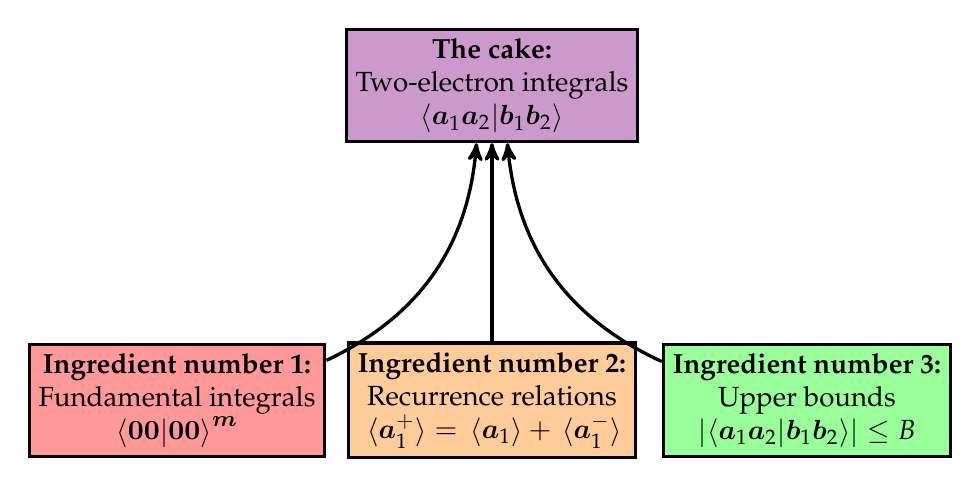
\begin{tikzpicture}
	\begin{scope}[very thick,
		node distance=4cm,on grid,>=stealth',
		boxRR/.style={rectangle,draw,fill=green!40},
		boxUB/.style={rectangle,draw,fill=orange!40},
		boxFI/.style={rectangle,draw,fill=red!40},
		integral/.style={rectangle,draw,fill=violet!40}],
		\node [integral, align=center]		(1)					{\textbf{The cake:} \\ Two-electron integrals \\ $\braket{\ba_1 \ba_2}{ \bb_1 \bb_2}$};
		\node [boxUB, align=center]		(2A)		[below=of 1]	{\textbf{Ingredient number 2:} \\ Recurrence relations \\ $\expval*{\ba_1^+} = \expval*{\ba_1} + \expval*{\ba_1^-}$};
		\node [boxRR, align=center] 		(2B)		[right=of 2A]	{\textbf{Ingredient number 3:} \\ Upper bounds \\ $\abs{\braket{\ba_1 \ba_2}{ \bb_1 \bb_2}} \le B$};
		\node [boxFI, align=center]		(2C)		[left=of 2A]	{\textbf{Ingredient number 1:} \\ Fundamental integrals \\ $\braket{\bo\bo}{\bo\bo}^{\bm{m}}$};
		\path 
		(1) edge [<-]			(2A)
		(1) edge [<-,bend right]			(2B)
		(1) edge [<-,bend left]					(2C)
		;
	\end{scope}
\end{tikzpicture}
\end{frame}

\begin{frame}{Late-contraction path algorithm (Head-Gordon-Pople \& PRISM inspired)}
	\begin{tikzpicture}
		\begin{scope}[
			very thick,
			node distance=1.5cm,on grid,>=stealth',
			boxSP/.style={rectangle,draw,fill=purple!40},
			box0m/.style={rectangle,draw,fill=red!40},
			boxCm/.style={rectangle,draw,fill=gray!40},
			boxA/.style={rectangle,draw,fill=red!40},
			boxAA/.style={rectangle,draw,fill=red!40},
			boxAAA/.style={rectangle,draw,fill=red!40},
			boxC/.style={rectangle,draw,fill=gray!40},
			boxCC/.style={rectangle,draw,fill=gray!40},
			boxCCC/.style={rectangle,draw,fill=orange!40},
			boxCCCCCC/.style={rectangle,draw,fill=green!40},
			],
			\node [boxSP, align=center]			(SP)									{Shell-pair \\ data};
			\node [box0m, align=center]			(0m)			[right=of 1,xshift=1.25cm]		{$\sbraket{00}{00}^{\bm{m}}$};
			\node [boxCm, align=center]			(Cm)			[right=of 0m,xshift=1.75cm]	{$\braket{00}{00}^{\bm{m}}$};
			\node [boxA, align=center] 			(A)			[below=of 0m]				{$\sbraket{0 a_2}{00}^{\bm{m}}$};
			\node [boxC, align=center] 			(C)			[right=of A,xshift=1.75cm]		{$\braket{0 a_2}{00}^{\bm{m}}$};
			\node [boxAA, align=center] 			(AA)			[below=of A]				{$\sbraket{a_1 a_2}{00}$};
			\node [boxCC, align=center] 			(CC)			[right=of AA,xshift=1.75cm]	{$\braket{a_1 a_2}{00}$};
			\node [boxCCCCCC, align=center] 		(CCCC)	[right=of CC,xshift=2cm]		{$\braket{a_1 a_2}{b_1 b_2}$};
			\path 
			(SP)		edge[->]			node[below,blue]{T$_0$}									(0m)
			(0m)		edge[->]			node[left,orange]{T$_1$}			node [right,red]{VRR$_1$}	(A)
			(0m)		edge[->,gray!70]														(Cm)
			(A)		edge[->]			node[left,orange]{T$_2$}			node [right,red]{VRR$_2$}	(AA)
			(A)		edge[->,gray!70]														(C)
			(AA)		edge[->]			node [below,blue]{CC}											(CC)
			(Cm)		edge[->,gray!70]														(C)
			(C)		edge[->,gray!70]														(CC)
			(CC)	edge[->]			node [above,orange]{T$_3$}		node [below,red]{HRR}		(CCCC)
			;
		\end{scope}
	\end{tikzpicture}
	\bigskip
	\begin{itemize}
		\item \red{HRR} = horizontal recurrence relation [Obara-Saika]
		\item \red{VRR} = vertical recurrence relation
		\item \blue{CC} = bra contraction
	\end{itemize}
\end{frame}

%\begin{frame}{Screening algorithm for two-electron integrals}
%
%\resizebox{\textwidth}{!}{
%\begin{tikzpicture}
%	\begin{scope}[very thick,
%		node distance=2.5cm,on grid,>=stealth',
%		bound2/.style={diamond,draw,fill=blue!40},
%		bound4/.style={diamond,draw,fill=blue!40},
%		bound6/.style={diamond,draw,fill=blue!40},
%		shell/.style={circle,draw,fill=green!40},
%		shellpair/.style={circle,draw,fill=green!40},
%		shellquartet/.style={circle,draw,fill=green!40},
%		shell1/.style={rectangle,draw,fill=yellow!40},
%		shell2/.style={rectangle,draw,fill=orange!40},
%		shell3/.style={rectangle,draw,fill=red!40},
%		integral/.style={rectangle,draw,fill=violet!40}],
%		\node [shell1, align=center]		(1)											{Primitive\\shells\\$\sket{a}$};
%		\node [bound2, align=center] 		(B2)			[right=of 1]				{$\sexpval{B_2}$};
%		\node [shell, align=center]			(S1T)		[above=of B2, yshift=-0.5cm]	{$\sket{a}$};
%		\node [shell, align=center]			(S1B)		[below=of B2, yshift=0.5cm]		{$\sket{b}$};
%		\node [shell2, align=center] 		(2)			[right=of B2,xshift=0.75cm]		{Contracted\\shell-pairs\\$\ket{ab}$};
%		\node [bound4, align=center]		(B4)			[right=of 2]				{$\expval{B_4}$} ;
%		\node [shellpair, align=center]		(S2T)		[above=of B4, yshift=-0.5cm]	{$\ket{a_1b_1}$};
%		\node [shellpair, align=center]		(S2B)		[below=of B4, yshift=0.5cm]		{$\ket{a_2b_2}$};
%		\node [shell3, align=center]		(3)			[right=of B4]					{Two-Electron\\integrals\\$\braket{a_1b_1}{a_2b_2}$};
%		\path 
%		(1) edge [->,bend left]				(S1T)
%		(1) edge [->,bend right]			(S1B)
%		(S1T) edge [snake it]				(B2)
%		(S1B) edge [snake it]				(B2)
%		(B2) edge [->,color=red] 	node [below] {\small Contraction}		(2)
%		(2) edge [->,bend left] 				(S2T)
%		(2) edge [->,bend right] 			(S2B)
%		(S2T) edge [snake it]				(B4)
%		(S2B) edge [snake it]				(B4)
%		(B4) edge [->] 					(3)
%		;
%	\end{scope}
%\end{tikzpicture}
%}
%\end{frame}

\begin{frame}{Orthogonalization matrix}
	\red{\bf We are looking for a matrix in order to orthogonalize the AO basis, i.e.~$\bm{X}^\dag \cdot \bm{S} \cdot  \bm{X} = \bm{1}$}
	\\
	\bigskip
	\begin{block}{Symmetric (or L\"owdin) orthogonalization}
		\begin{equation}
			\text{$\bm{X} =\bm{S}^{-1/2} = \bm{U} \cdot  \bm{s}^{-1/2} \cdot  \bm{U}^\dag$ is one solution...}
		\end{equation}
		\purple{\bf Is it working?}
		\begin{equation}
			\bm{X}^\dag \cdot \bm{S} \cdot \bm{X} 
			= \bm{S}^{-1/2} \cdot \bm{S} \cdot \bm{S}^{-1/2} 
			= \bm{S}^{-1/2} \cdot \bm{S} \cdot \bm{S}^{-1/2} 
			= \bm{I} \quad \green{\checkmark}
		\end{equation}
	\end{block}
	\begin{block}{Canonical orthogonalization}
		\begin{equation}
			\text{$\bm{X} =\bm{U} \cdot \bm{s}^{-1/2}$ is another solution (when you have linear dependencies)...}
		\end{equation}
			\purple{\bf Is it working?}
		\begin{equation}
			\bm{X}^\dag \cdot \bm{S} \cdot  \bm{X} 
			= \bm{s}^{-1/2} \cdot \underbrace{\bm{U}^{\dag} \cdot \bm{S} \cdot \bm{U}}_{\bm{s}} \cdot \bm{s}^{-1/2} 
			= \bm{I} \quad \green{\checkmark}
		\end{equation}
	\end{block}
\end{frame}

\begin{frame}{Computation of the Fock matrix and energy}
	\begin{block}{Density matrix (closed-shell system)}
		\begin{equation}
			 P_{\red{\mu \nu}} = 2 \sum_{i}^\text{occ} C_{\red{\mu} i} C_{\red{\nu} i}
			\qqtext{or} 
			\boxed{\bm{P} = \bm{C} \cdot \bm{C}^{\dag}}
		\end{equation}
	\end{block}
	\begin{block}{Fock matrix in the AO basis (closed-shell system)}
		\begin{equation}
			F_{\red{\mu\nu}} 
			= H_{\red{\mu\nu}} 
			+ \underbrace{\sum_{\blue{\la \si}} P_{\blue{\la\si}} (\red{\mu\nu}|\blue{\la\si})}_{J_{\red{\mu \nu}} = \text{ Coulomb}}
			\underbrace{ - \frac{1}{2} \sum_{\blue{\la \si}} P_{\blue{\la\si}} (\red{\mu}\blue{\si}|\blue{\la}\red{\nu})}_{K_{\red{\mu \nu}} = \text{ exchange}}
		\end{equation}
	\end{block}
	\begin{block}{HF energy in the AO basis (closed-shell system)}
		\begin{equation}
			E_\text{HF} = \sum_{\red{\mu \nu}} P_{\red{\mu \nu}} H_{\red{\mu \nu}} 
			+ \frac{1}{2} \sum_{\red{\mu \nu} \blue{\la\si}} P_{\red{\mu \nu}} \qty[ (\red{\mu \nu} | \blue{\lambda \sigma}) - \frac{1}{2} (\red{\mu} \blue{\sigma} | \red{\lambda} \blue{\nu}) ] P_{\blue{\lambda\sigma}}
			\qqtext{or} 
			\boxed{E_\text{HF} = \frac{1}{2} \text{Tr}{\qty[\bm{P} \cdot (\bm{H} + \bm{F})]}}
		\end{equation}
	\end{block}
\end{frame}

\begin{frame}{Computation of the Fock matrix and energy}
	\begin{algorithmic}
		\Procedure{Computing the Coulomb matrix}{}
			\For{$\red{\mu}=1,N$}
				\For{$\blue{\nu}=1,N$}
					\State $J_{\red{\mu}\blue{\nu}} = 0$ \Comment{Initialization of the array}
					\For{$\orange{\la}=1,N$}
						\For{$\violet{\si}=1,N$}
							\State $J_{\red{\mu}\blue{\nu}} 
							= J_{\red{\mu}\blue{\nu}} 
							+ P_{\orange{\la}\violet{\si}} (\red{\mu}\blue{\nu}|\orange{\la}\violet{\si})$ 
							\Comment{Accumulation step}
						\EndFor
					\EndFor 
				\EndFor
			\EndFor 
		\EndProcedure
		\Comment{\bf \red{This is a $\order{N^4}$ algorithm as it involves four loops}}
	\end{algorithmic}
\end{frame}

%%% SLIDE X %%%
\begin{frame}{Resolution of the identity}
	\begin{block}{Resolution of the identity (RI)}
		\begin{equation}
			\sum_{\green{A}=1}^{\red{\infty}} \dyad{\green{A}} = \hI
			\qq{with}
			\braket{\green{A}}{\green{B}} = \delta_{AB}
			\qq{$\Leftrightarrow$}
			\sum_{\green{A}=1}^{\red{\infty}} \green{A}(\br_1) \green{A}(\br_2)  
			= \delta(\br_1 - \br_2) 
		\end{equation}
	\end{block}
	\begin{block}{Generalization to a two-body operator $\hO$}
		\begin{equation}
			\sum_{\green{\Tilde{A}}=1}^{\red{\infty}} \dyad{\green{\Tilde{A}}} = \hO
			\qq{with}
			\mel{\green{A}}{\hO}{\green{B}} = \delta_{AB}
			\qq{and}
			\hO \ket{\green{A}} = \ket{\green{\Tilde{A}}}
			\qq{$\Leftrightarrow$}
			\sum_{\green{\Tilde{A}}=1}^{\red{\infty}} \green{\Tilde{A}}(\br_1) \green{\Tilde{A}}(\br_2)  
			= \hO(\br_1,\br_2) 
		\end{equation}
	\end{block}
\end{frame}
%

%%% SLIDE X %%%
\begin{frame}{Resolution of the Coulomb operator}
	\begin{block}{RI in practice = RI \alert{approximation}}
		\begin{equation}
			\boxed{\sum_{\green{A}=1}^{\red{\infty}} \dyad{\green{A}} = \hI 
			\qqtext{and, in practice, }
			\sum_{\green{A}=1}^{\red{K}} \dyad{\green{A}} \approx \hI}
		\end{equation}
	\end{block}
	\begin{block}{Computing the Coulomb matrix within the RI approximation}
		\begin{equation}
			\begin{split}
				J_{\red{\mu\nu}} 
				& = \sum_{\blue{\la \si}} P_{\blue{\la\si}} (\red{\mu\nu}|\blue{\la\si})
				\\
				& \stackrel{\text{\green{RI}}}{=}  \sum_{\blue{\la \si}} P_{\blue{\la\si}} \sum_{\green{A}} (\red{\mu\nu}|\green{A}) (\green{A}|\blue{\la\si})
				\\
				& = \sum_{\green{A}} (\red{\mu\nu}|\green{A})  
				\underbrace{\sum_{\blue{\la \si}} P_{\blue{\la\si}} (\green{A}|\blue{\la\si})}_{\order{KN^2} \text{ and $K$ storage}}
				= \underbrace{\sum_{\green{A}} (\red{\mu\nu}|\green{A})  \rho_{\green{A}}}_{\order{KN^2}}
			\end{split}
		\end{equation}
		\\
		Similar (more effective) approaches are named Cholesky decomposition, low-rank approximation, etc. 
	\end{block}
\end{frame}
%

\begin{frame}{Computation of exact exchange}
	\begin{algorithmic}
		\Procedure{Computing the exchange matrix}{}
			\For{$\red{\mu}=1,N$}
				\For{$\blue{\nu}=1,N$}
					\State $K_{\red{\mu}\blue{\nu}} = 0$ \Comment{Initialization of the array}
					\For{$\orange{\la}=1,N$}
						\For{$\violet{\si}=1,N$}
							\State $K_{\red{\mu}\blue{\nu}} 
							= K_{\red{\mu}\blue{\nu}} 
							+ P_{\orange{\la}\violet{\si}} (\red{\mu}\violet{\si}|\orange{\la}\blue{\nu})$ 
							\Comment{Accumulation step}
						\EndFor
					\EndFor 
				\EndFor
			\EndFor 
		\EndProcedure
		\Comment{\bf \red{This is a $\order{N^4}$ algorithm and it's hard to play games...}}
	\end{algorithmic}
\end{frame}

\begin{frame}{Computation of DFT exchange}
	\begin{block}{LDA exchange (in theory) = cf \sout{Julien's} Manu's lectures}
		\begin{gather}
			K_{\mu\nu}^\text{LDA} 
			= \int \phi_{\mu}(\br) \violet{v_\text{x}^\text{LDA}}(\br) \phi_{\nu}(\br)  d\br 
			= \frac{4}{3} C_\text{x}  \overbrace{\int \phi_{\mu}(\br) \blue{\rho^{1/3}}(\br) \phi_{\nu}(\br) d\br}^{\text{\alert{no closed-form expression in general}}}
			\\
			\blue{\rho}(\br) = \sum_{\mu \nu} \phi_{\mu}(\br) \blue{P_{\mu \nu}} \phi_{\nu}(\br)
		\end{gather}
	\end{block}
	\begin{block}{LDA exchange (in practice) = \alert{numerical integration via quadrature} = $\int f(x) dx \approx \sum_k w_k f(x_k)$}
		\begin{gather}
			\underbrace{K_{\mu\nu}^\text{LDA}}_{\green{\order{N_\text{grid} N^2}}}
			\approx \sum_{k=1}^{\purple{N_\text{grid}}} 
			\underbrace{\orange{w_k}}_{\orange{\text{weights}}} \phi_{\mu}(\red{\br_k}) \violet{v_\text{x}^\text{LDA}}(\underbrace{\red{\br_k}}_{\text{\red{roots}}}) \phi_{\nu}(\red{\br_k}) 
			= \frac{4}{3} C_\text{x} \sum_{k=1}^{\purple{N_\text{grid}}} \orange{w_k} \phi_{\mu}(\red{\br_k}) \blue{\rho^{1/3}}(\red{\br_k}) \phi_{\nu}(\red{\br_k})
			\\
			\underbrace{\blue{\rho}(\red{\br_k})}_{\green{\order{N_\text{grid} N^2}}} = \sum_{\mu \nu} \phi_{\mu}(\red{\br_k}) \blue{P_{\mu \nu}} \phi_{\nu}(\red{\br_k})
		\end{gather}
	\end{block}
\end{frame}


\begin{frame}{The correlation energy}
	\begin{itemize}
		\item HF replaces the e-e interaction by an \green{averaged interaction}
		\bigskip
		\item The error in the HF method is called the \purple{correlation energy}
		$$\boxed{E_c = E - E_\text{HF}} $$
		\item The correlation energy is small \orange{but cannot but neglected!}
		\bigskip
		\item HF energy \blue{roughly 99\%} of total but \blue{chemistry very sensitive to remaining 1\%}
		\bigskip
		\item The correlation energy is \alert{always negative}
		\bigskip
		\item Computing $E_c$ is one of the \violet{central problem of quantum chemistry}
		\bigskip
		\item In quantum chemistry, we usually \alert{``freeze'' the core electrons} for correlated calculations
	\end{itemize}
\end{frame}

\begin{frame}{Most common correlation methods in quantum chemistry}
	\begin{enumerate}
		\item \alert{Configuration Interaction}: CID, CIS, CISD, CISDTQ, etc.
		\bigskip
		\item \alert{Coupled Cluster}: CCD, CCSD, CCSD(T), CCSDT, CCSDTQ, etc.
		\bigskip
		\item \alert{M{\o}ller-Plesset perturbation theory}: MP2, MP3, MP4, MP5, etc.
		\bigskip
		\item \alert{Multireference methods}: MCSCF, CASSCF, RASSCF, MRCI, MRCC, CASPT2, NEVPT2, etc. (C.~Angeli \& S. Knecht)
		\bigskip
		\item \alert{Density-functional theory}: DFT, TDDFT, etc. (J. Toulouse/E. Fromager, F. Sottile)
		\bigskip
		\item \alert{Quantum Monte Carlo}: VMC, DMC, FCIQMC, etc. (M.~Caffarel)
	\end{enumerate}
\end{frame}

\begin{frame}{Configuration Interaction (CI)}
	\begin{itemize}
		\item This is the \blue{oldest} and perhaps the \blue{easiest method to understand}
		\bigskip
		\item CI is based on the \orange{variational principle} (like HF)
		\bigskip
		\item The CI wave function is a \blue{linear combination of determinants}
		\bigskip
		\item CI methods use \violet{excited determinants} to ``improve'' the reference (usually HF) wave function
			\begin{equation}
				\ket{\Phi_0} 
				= \underbrace{c_0 \ket*{\Psi_0}}_{\text{reference}}
				+ \underbrace{\violet{\sum_{\substack{i \\ a}} c_i^a \ket*{\Psi_i^a}}}_{\text{singles}}
				+ \underbrace{\purple{\sum_{\substack{i < j \\ a < b}}  c_{ij}^{ab} \ket*{\Psi_{ij}^{ab}}}}_{\text{doubles}}
				+ \underbrace{\orange{\sum_{\substack{i < j < k \\ a < b < c}}  c_{ijk}^{abc} \ket*{\Psi_{ijk}^{abc}}}}_{\text{triples}}
				+ \underbrace{\blue{\sum_{\substack{i < j < k < l \\ a < b < c < d}}  c_{ijkl}^{abcd} \ket*{\Psi_{ijkl}^{abcd}}}}_{\text{quadruples}} 
				+ \ldots
			\end{equation}
	\end{itemize}
\end{frame}

\begin{frame}{CI method and Excited determinants}
	\begin{block}{Excited determinants}
		\center
		\includegraphics[width=0.7\textwidth]{fig/det}
	\end{block}
	\begin{block}{CI wave function}
		\begin{equation}
		\boxed{ 
			\ket{\Phi_0} 
			= c_0 \ket{\text{0}} 
			+ \violet{c_\text{S} \ket{\text{S}}} 
			+ \purple{c_\text{D} \ket{\text{D}}} 
			+ \orange{c_\text{T} \ket{\text{T}}} 
			+ \blue{c_\text{Q} \ket{\text{Q}}} 
			+ \ldots 
			}
		\end{equation}
	\end{block}
\end{frame}


\begin{frame}{Excited determinants}
	\begin{block}{Reference determinant}	
		\begin{equation}
			\qq*{\green{The electrons are in the $N$ lowest spinorbitals (Aufbau principle):}} \ket{\Psi_0} \equiv \ket{0} = \ket{\chi_1 \ldots \chi_{\green{i}} \chi_{\green{j}} \ldots \chi_N}
		\end{equation}
	\end{block}
	\begin{block}{Singly-excited determinants}	
		\begin{equation}
			\qq*{Electron in $\green{i}$ promoted in $\red{a}$:} \ket{\Psi_{\green{i}}^{\red{a}}} = \ket{\chi_1 \ldots \chi_{\red{a}} \chi_{\green{j}} \ldots \chi_N}
		\end{equation}
	\end{block}
	\begin{block}{Doubly-excited determinants}	
		\begin{equation}
			\qq*{Electrons in $\green{i}$ and $\green{j}$ promoted in $\red{a}$ and $\red{b}$:} \ket{\Psi_{\green{ij}}^{\red{ab}}} = \ket{\chi_1 \ldots \chi_{\red{a}} \chi_{\red{b}} \ldots \chi_N}
		\end{equation}
	\end{block}
%	\begin{center}
%		\includegraphics[width=0.15\textwidth]{fig/GS}
%		\hspace{0.2\textwidth}
%		\includegraphics[width=0.15\textwidth]{fig/single}
%		\hspace{0.2\textwidth}
%		\includegraphics[width=0.15\textwidth]{fig/double}
%	\end{center}
\end{frame}


\begin{frame}{Truncated CI}
	\begin{itemize}
		\item When $\ket{\text{S}}$ (\violet{singles}) are taken into account: \textbf{CIS}
			\begin{equation}
				\violet{\ket{\Phi_\text{CIS}} = c_0 \ket{\text{0}} + c_\text{S} \ket{\text{S}}}
			\end{equation}
			\textbf{NB:} CIS is an \violet{excited state method}
		\item When $\ket{\text{D}}$ (\alert{doubles}) are taken into account: \textbf{CID}
			\begin{equation}
				\alert{\ket{\Phi_\text{CID}} = c_0 \ket{\text{0}} + c_\text{D} \ket{\text{D}}}
			\end{equation}
			\textbf{NB:} CID is the \alert{cheapest CI method}
		\item When $\ket{\text{S}}$  and $\ket{\text{D}}$ are taken into account: \textbf{CISD}
			\begin{equation}
			\purple{\ket{\Phi_\text{CISD}} = c_0 \ket{\text{0}} + c_\text{S} \ket{\text{S}} + c_\text{D} \ket{\text{D}} }
			\end{equation}
			\textbf{NB:} CISD is the \purple{most commonly-used} CI method
		\item When $\ket{\text{S}}$, $\ket{\text{D}}$ and $\ket{\text{T}}$ (\orange{triples}) are taken into account: \textbf{CISDT}
			\begin{equation}
				\orange{\ket{\Phi_\text{CISDT}} = c_0 \ket{\text{0}} + c_\text{S} \ket{\text{S}} + c_\text{D} \ket{\text{D}} + c_\text{T} \ket{\text{T}}}
			\end{equation}
		\item \textbf{CISDTQ}, etc.
	\end{itemize}
\end{frame}

\begin{frame}{Full CI}
	\begin{itemize}
		\item When all possible excitations are taken into account,
		 \alert{this is called a Full CI calculation} (\textbf{FCI})
			\begin{equation}
				\alert{\ket{\Phi_\text{FCI}} 
				= c_0 \ket{\text{0}} 
				+ c_\text{S} \ket{\text{S}} 
				+ c_\text{D} \ket{\text{D}} 
				+ c_\text{T} \ket{\text{T}} 
				+ c_\text{Q} \ket{\text{Q}}
				+ \ldots}
			\end{equation}
		\item FCI gives the \violet{exact solution of the Schr\"odinger equation within a given basis}
		\bigskip
		\item FCI is becoming more and more fashionable these days (e.g. \orange{FCIQMC and SCI methods})
		\bigskip
		\item \blue{So, why do we care about other methods?}
		\bigskip
		\item \alert{Because FCI is super computationally expensive!}
		\bigskip
	\end{itemize}
\end{frame}


\begin{frame}{Size of CI Matrix}
	\violet{\textit{``Assume we have 10 electrons in 38 spin MOs: 10 are occupied and 28 are empty''}}
	\bigskip
	\begin{columns}
		\begin{column}{0.65\textwidth}
				\begin{itemize}
					\item There is $C_{10}^k$ possible ways of selecting $k$ electrons out of the 10 occupied orbitals 
					$$ C_{n}^k = \frac{n!}{k!(n-k)!} $$
					\item There is $C_{28}^k$ ways of distributing them out in the 28 virtual orbitals
					\item For a given excitation level $k$, \alert{there is $C_{10}^k C_{28}^k$ excited determinants}
					\item \violet{The total number of possible excited determinant} is 
					$$ \sum_{k=0}^{10}C_{10}^k C_{28}^k = C_{38}^{10} = 472,733,756$$
					\item \alert{This is a lot...}
				\end{itemize}
		\end{column}
		\begin{column}{0.35\textwidth}
			\small
			\orange{For $n = 10$ and $N = 38$:}
			\\
			\bigskip
			\begin{tabular}{cr}
				\hline \hline
				$k$	&	Num. of excitations	\\
				\hline
				0 	& 	1 			\\
 	 	 		1 	&	280 			\\
 	 	 		2 	&	17,010		\\
 	 	 		3 	&	393,120 		\\
 	 	 		4 	&	4,299,750 	\\
 	 	 		5 	&	24,766,560	\\
 	 	 		6 	&	79,115,400 	\\
 	 	 		7 	&	142,084,800	\\
 	 	 		8 	&	139,864,725	\\
 	 	 		9 	&	69,069,000	\\
				10 	&	13,123,110	\\
				\hline
				Tot. 	&	472,733,756	\\
				\hline \hline
			\end{tabular}
		\end{column}
	\end{columns}
\end{frame}
\begin{frame}{Pople diagram}
	\centering
	\includegraphics[width=0.7\textwidth]{fig/pople_CI}
\end{frame}

\begin{frame}{CI Lagrangian}
	The CI Lagrangian is 
	\begin{equation}
		L = \mel{\Phi_\text{CI}}{\hH}{\Phi_\text{CI}} - \la \qty( \braket{\Phi_\text{CI}}{\Phi_\text{CI}} - 1)
		\qq{with}
		\ket{\Phi_\text{CI}} = \sum_I c_I \ket{I}
	\end{equation}
	with
	\begin{gather}
		\mel{\Phi_\text{CI}}{\hH}{\Phi_\text{CI}} 
		= \sum_{IJ} c_I c_J \mel{I}{\hH}{J} 
		= \sum_I c_I^2 \underbrace{\mel{I}{\hH}{I}}_{H_{II}} + \sum_{I \neq J} \underbrace{\mel{I}{\hH}{J}}_{H_{IJ}}
		\\
		\braket{\Phi_\text{CI}}{\Phi_\text{CI}} 
		= \sum_{IJ} c_I c_J \braket{I}{J} 
		= \sum_{I} c_I^2
	\end{gather}
	Following the variational procedure, we get
	\begin{equation}
		\pdv{L}{c_I} = 2 \sum_J c_J H_{IJ} - 2 \la c_I = 0
		\qq{or}
		\boxed{\qty( H_{II} - \la) c_I + \sum_{J \neq I} H_{IJ} c_J = 0}
	\end{equation}
\end{frame}

\begin{frame}{CI secular equations}
	\begin{equation}
		\begin{pmatrix}
    		H_{00} - E 	&	H_{01}		&	\hdots	&	H_{0J}		&	\hdots	\\
    		H_{10}		&	H_{11} - E	&	\hdots	&	H_{1J}		&	\hdots	\\
    		\vdots		&	\vdots		&	\ddots	&	\vdots		&	\hdots	\\
    		H_{J0}		&	\vdots		&	\hdots	&	H_{JJ} - E	&	\hdots	\\
    		\vdots		&	\vdots		&	\hdots	&	\vdots		&	\ddots	\\
		\end{pmatrix}
		\begin{pmatrix}
    		c_{0}	\\
    		c_{1}	\\
    		\vdots	\\
    		c_{J}	\\
    		\vdots	\\
		\end{pmatrix}
		= 
		\begin{pmatrix}
    		0 		\\
    		0		\\
    		\vdots	\\
    		0		\\
    		\vdots	\\
		\end{pmatrix}
		\qq{or}
		\boxed{\bH \cdot \bc = E \bc}
	\end{equation}
\end{frame}

\begin{frame}{The FCI matrix: \alert{before pruning}}
	\begin{equation}
		\boxed{
			\ket{\Phi_0} 
			= c_0 \ket{\text{HF}} 
			+ c_\text{S} \ket{\text{S}} 
			+ c_\text{D} \ket{\text{D}} 
			+ c_\text{T} \ket{\text{T}} 
			+ c_\text{Q} \ket{\text{Q}} 
			+ \ldots
		}
	\end{equation}
	\bigskip
	\begin{equation}
	\bH = 
	\begin{array}{ccccccc}
						&	| \text{HF} \rangle						&	 | \text{S} \rangle							&	| \text{D} \rangle							&	| \text{T} \rangle							&	 | \text{Q} \rangle							&	\cdots	\\
		\langle \text{HF}  |	&	\langle \text{HF}	 | \hH | \text{HF} \rangle	&	\langle \text{HF}	 | \hH | \text{S} \rangle 		&	\langle \text{HF}	 | \hH | \text{D} \rangle		&	\langle \text{HF}	 | \hH | \text{T} \rangle		&	\langle \text{HF}	 | \hH | \text{Q} \rangle		&	\cdots		\\
		\langle \text{S} |	&	\langle \text{S} | \hH | \text{HF} \rangle	&	\langle \text{S} | \hH | \text{S} \rangle 	&	\langle \text{S} | \hH | \text{D} \rangle		&	\langle \text{S} | \hH | \text{T} \rangle		&	\langle \text{S} | \hH | \text{Q} \rangle		&	\cdots		\\
		\langle \text{D} |	&	\langle \text{D} | \hH |\text{HF} \rangle	&	\langle \text{D} | \hH | \text{S} \rangle 	&	\langle \text{D} | \hH | \text{D} \rangle		&	\langle \text{D} | \hH| \text{T} \rangle		&	\langle \text{D} | \hH | \text{Q} \rangle	&	\cdots		\\
		\langle \text{T} |	&	\langle \text{T} | \hH |\text{HF} \rangle	&	\langle \text{T} | \hH | \text{S} \rangle 	&	\langle \text{T} | \hH | \text{D} \rangle		&	\langle \text{T} |\hH | \text{T} \rangle		&	\langle \text{T} | \hH | \text{Q} \rangle		&	\cdots		\\
		\langle \text{Q} |	&	\langle \text{Q} | \hH | \text{HF} \rangle	&	\langle \text{Q} | \hH | \text{S} \rangle 	&	\langle \text{Q} | \hH | \text{D} \rangle	&	\langle \text{Q} | \hH | \text{T} \rangle		&	\langle \text{Q} | \hH | \text{Q} \rangle	&	\cdots		\\
		\vdots			&	\vdots								&	\vdots									&	\vdots									&	\vdots									&	\vdots									&	\vdots		\\
	\end{array}
	\end{equation}
\end{frame}
\begin{frame}{The FCI matrix: \green{after pruning}}
	\begin{equation}
		\boxed{
			\ket{\Phi_0} 
			= c_0 \ket{\text{HF}} 
			+ c_\text{S} \ket{\text{S}} 
			+ c_\text{D} \ket{\text{D}} 
			+ c_\text{T} \ket{\text{T}} 
			+ c_\text{Q} \ket{\text{Q}} 
			+ \ldots
		}
	\end{equation}
	\bigskip
	\begin{equation}
	\bH = 
	\begin{array}{ccccccc}
						&	| \text{HF} \rangle						&	 | \text{S} \rangle							&	| \text{D} \rangle							&	| \text{T} \rangle							&	 | \text{Q} \rangle							&	\cdots	\\
		\langle \text{HF}	 |	&	\langle \text{HF}	 | \hH | \text{HF} \rangle	&	0								 		&	\langle \text{HF}	 | \hH | \text{D} \rangle		&	0										&	0										&	\cdots		\\
		\langle \text{S} |	&	0									&	\langle \text{S} | \hH | \text{S} \rangle 	&	\langle \text{S} | \hH | \text{D} \rangle		&	\langle \text{S} | \hH | \text{T} \rangle		&	0										&	\cdots		\\
		\langle \text{D} |	&	\langle \text{D} | \hH | \text{HF} \rangle	&	\langle \text{D} | \hH | \text{S} \rangle 	&	\langle \text{D} | \hH | \text{D} \rangle		&	\langle \text{D} | \hH | \text{T} \rangle		&	\langle \text{D} | \hH | \text{Q} \rangle	&	\cdots		\\
		\langle \text{T} |	&	0									&	\langle \text{T} | \hH | \text{S} \rangle 	&	\langle \text{T} | \hH | \text{D} \rangle		&	\langle \text{T} | \hH | \text{T} \rangle		&	\langle \text{T} | \hH | \text{Q} \rangle		&	\cdots		\\
		\langle \text{Q} |	&	0									&	0										&	\langle \text{Q} | \hH | \text{D} \rangle	&	\langle \text{Q} | \hH | \text{T} \rangle		&	\langle \text{Q} | \hH | \text{Q} \rangle	&	\cdots		\\
		\vdots			&	\vdots								&	\vdots									&	\vdots									&	\vdots									&	\vdots									&	\vdots		\\
	\end{array}
	\end{equation}
\end{frame}

\begin{frame}{Rules \& Observations}
	\begin{enumerate}
		\item No coupling between HF ground state $\ket{ \text{HF} }$ and single excitations $ \ket{ \text{S} }$\\
			\violet{$\Rightarrow$ Brillouin's theorem} 
    		\begin{equation}
    			\violet{\mel{ \text{HF} }{ \hH }{ \text{S} } = 0}
    		\end{equation}
		\item No coupling between $\ket{ \text{HF} }$ and triples $\ket{ \text{T} }$ , quadruples $ \ket{ \text{Q} }$ , etc. \\
			\alert{$\Rightarrow$ Slater-Condon rules}
    		\begin{gather}
    			\alert{\mel{ \text{HF} }{ \hH }{ \text{T} } = \mel{ \text{HF} }{ \hH }{ \text{Q} } = \ldots = 0}
    			\\
    			\alert{\mel{ \text{S} }{ \hH }{ \text{Q} } =  \ldots = 0} 
    		\end{gather}
		\item $ \ket{ \text{S} }$ have small effect but mix indirectly with $\ket{ \text{D} }$\\
			\orange{$\Rightarrow$ CID $\neq$ CISD}
    		\begin{equation}
    			\orange{\mel{ \text{HF} }{ \hH }{ \text{S} } = 0 \qq{but} \mel{ \text{S} }{ \hH }{ \text{D} } \neq 0}
    		\end{equation}
		 \item $ \ket{ \text{D} }$ have large effect and $ \ket{ \text{Q} }$ more important than $ \ket{ \text{T} }$\\
			\blue{$\Rightarrow$ CID gives most of the correlation energy}
    		\begin{equation}
    			\blue{\mel{ \text{HF} }{ \hH }{ \text{D} } \gg \mel{ \text{HF} }{ \hH }{ \text{Q} } \gg \mel{ \text{HF} }{ \hH }{ \text{T} }}
    		\end{equation}
		\item \purple{Of course, this matrix is never explicitly built in practice (Davidson algorithm)...}
	\end{enumerate}
\end{frame}

\begin{frame}{Slater-Condon rules: One-electron operators}
	\begin{equation}
		\boxed{\cO_1 = \sum_i^N h(i)}
	\end{equation}
	\begin{block}{\green{Case 1 = differ by zero spinorbital}: $\ket{K} = \ket{\cdots ij \cdots}$}
		\begin{equation}
			\mel{K}{\cO_1}{K} = \sum_i^N \mel{i}{h}{i}
		\end{equation}
	\end{block}
	\begin{block}{\orange{Case 2 = differ by one spinorbital}: $\ket{K} = \ket{\cdots ij \cdots}$ and $\ket{L} = \ket{\cdots aj \cdots}$}
		\begin{equation}
			\mel{K}{\cO_1}{L} = \mel{i}{h}{a}
		\end{equation}
	\end{block}
	\begin{block}{\red{Case 3 = differ by two spinorbitals}: $\ket{K} = \ket{\cdots ij \cdots}$ and $\ket{L} = \ket{\cdots ab \cdots}$}
		\begin{equation}
			\mel{K}{\cO_1}{L} = 0
		\end{equation}
	\end{block}
\end{frame}

\begin{frame}{Slater-Condon rules: Two-electron operators}
	\begin{equation}
		\boxed{\cO_2 = \sum_{i<j}^N r_{ij}^{-1}}
	\end{equation}
	\begin{block}{\green{Case 1 = differ by zero spinorbital}: $\ket{K} = \ket{\cdots ij \cdots}$}
		\begin{equation}
			\mel{K}{\cO_2}{K} = \frac{1}{2} \sum_{ij}^N \mel{ij}{}{ij}
		\end{equation}
	\end{block}
	\begin{block}{\orange{Case 2 = differ by one spinorbital}: $\ket{K} = \ket{\cdots ij \cdots}$ and $\ket{L} = \ket{\cdots aj \cdots}$}
		\begin{equation}
			\mel{K}{\cO_2}{L} = \sum_j^N \mel{ij}{}{aj}
		\end{equation}
	\end{block}
	\begin{block}{\red{Case 3 = differ by two spinorbitals}: $\ket{K} = \ket{\cdots ij \cdots}$ and $\ket{L} = \ket{\cdots ab \cdots}$}
		\begin{equation}
			\mel{K}{\cO_2}{L} = \mel{ij}{}{ab}
		\end{equation}
	\end{block}
\end{frame}

\begin{frame}{Example}
	\begin{columns}
		\begin{column}{0.5\textwidth}
			\begin{block}{Weights of excited configurations for \ce{Ne}}
				\center
				\begin{tabular}{cc}
					\hline \hline
					Excit. level	&	Weight	\\
					\hline
					0 			& 	$9.6 \times 10^{-1}$	\\
 	 	 	 	 	1 			& 	$9.8 \times 10^{-4}$		\\
 	 	 	 	 	2 			& 	$3.4 \times 10^{-2}$		\\
 	 	 	 	 	3 			& 	$3.7 \times 10^{-4}$		\\
 	 	 	 	 	4 			& 	$4.5 \times 10^{-4}$		\\
 	 	 	 	 	5 			& 	$1.9 \times 10^{-5}$		\\
 	 	 	 	 	6 			& 	$1.7 \times 10^{-6}$		\\
 	 	 	 	 	7 			& 	$1.4 \times 10^{-7}$		\\
 	 	 	 	 	8 			& 	$1.1 \times 10^{-9}$		\\
					\hline \hline
				\end{tabular}
			\end{block}
		\end{column}
		\begin{column}{0.5\textwidth}
			\begin{block}{Correlation energy of \ce{Be} and Method scaling}
				\center
				\begin{table}
					\begin{tabular}{lccc}
					\hline \hline
						Method	&	$\Delta E_c$	&	\%		&	Scaling	\\
						\hline
						HF		&	0			&	0		&	$N^4$	\\
						CIS		&	0			&	0		&	$N^5$	\\
						CISD	&	0.075277		&	96.05	&	$N^6$	\\
						CISDT	&	0.075465		&	96.29	&	$N^8$	\\
						CISDTQ	&	0.078372		&	100		&	$N^{10}$	\\			
						FCI		&	0.078372		&	100		&	$e^N$	\\			
					\hline \hline
					\end{tabular}
				\end{table}
			\end{block}
		\end{column}
	\end{columns}
\end{frame}

\begin{frame}{Size consistency and size extensivity}
	\begin{itemize}
		\item Truncated CI methods are \alert{size inconsistent} 
		\bigskip
		\item Size consistent defines for \alert{non-interacting fragment}:
		\begin{equation*}
			\boxed{\qq{Let $A$ and $B$ be non-interacting systems, then} E(A+B) = E(A) + E(B)}
		\end{equation*}
		\item \alert{Size extensivity} refers to the scaling of $E_c$ with the number of electrons (i.e.~the system size)
		\bigskip
		\item Size consistency is of particular importance to obtaining correct \alert{dissociation curves}
		\bigskip
		\item  \alert{NB:} FCI is size consistent and size extensive
	\end{itemize}
\end{frame}

\begin{frame}{Rayleigh-Schr\"odinger perturbation theory}
	Let's assume we want to find $\Psi_0$ and $E_0$, such as 
	\begin{equation}
		(\hH^{(0)} + \alert{\la} \hH^{(1)}) \Psi_0 = E_0\,\Psi_0
	\end{equation}
	and that we know
	\begin{equation}
		\boxed{ \hH^{(0)} \Psi^{(0)}_n = E^{(0)}_n \Psi_n^{(0)}, \quad n = 0,1,2,\ldots,\infty}
	\end{equation}
	Let's expand $\Psi_0$ and $E_0$ in term of $\la$:
	\begin{equation}
		E_0 = \orange{\la^0}\,E_0^{(0)} + \red{\la^1}\,E_0^{(1)} + \purple{\la^2}\,E_0^{(2)} + \violet{\la^3}\,E_0^{(3)} + \ldots 
	\end{equation}
	\begin{equation}
		\Psi_0 = \orange{\la^0}\,\Psi_0^{(0)} + \red{\la^1}\,\Psi_0^{(1)} + \purple{\la^2}\,\Psi_0^{(2)} + \violet{\la^3}\,\Psi_0^{(3)} + \ldots 
	\end{equation}
	such as (\alert{intermediate normalization})
	\begin{equation}
		\braket*{ \Psi_0^{(0)} }{ \Psi_0^{(0)} } = 1 	\qquad 	\braket*{ \Psi_0^{(0)} }{ \Psi_0^{(k)} } = 0, \quad k = 1,2,\ldots,\infty
	\end{equation}
\end{frame}

\begin{frame}{Rayleigh-Schr\"odinger perturbation theory (Part 1)}
	Gathering terms with respect to the power of $\la$: 
	\begin{align}
		& \orange{\la^0:}	 \qquad	\hH^{(0)}\Psi_0^{(0)} = E_0^{(0)} \Psi_0^{(0)} 	
		\\
		& \red{\la^1:}	 	\qquad	\hH^{(0)}\Psi_0^{(1)} + \hH^{(1)}\Psi_0^{(0)} = E_0^{(0)} \Psi_0^{(1)} + E_0^{(1)} \Psi_0^{(0)}	
		\\
		& \purple{\la^2:}	 \qquad	\hH^{(0)}\Psi_0^{(2)} + \hH^{(1)}\Psi_0^{(1)} = E_0^{(0)} \Psi_0^{(2)} + E_0^{(1)} \Psi_0^{(1)} + E_0^{(2)} \Psi_0^{(0)}			
		\\ 
		& \violet{\la^3:}	 \qquad	\hH^{(0)}\Psi_0^{(3)} + \hH^{(1)}\Psi_0^{(2)} = E_0^{(0)} \Psi_0^{(3)} + E_0^{(1)} \Psi_0^{(2)} + E_0^{(2)} \Psi_0^{(1)} + E_0^{(3)} \Psi_0^{(0)}	
	\end{align} 
	Using the intermediate normalization, we have
	\begin{align}
		&  \orange{\la^0:}	 \qquad	E_0^{(0)} = \mel*{ \Psi_0^{(0)} }{ \hH^{(0)} }{ \Psi_0^{(0)} }	
		\\
		& \red{\la^1:}		 \qquad	E_0^{(1)} = \mel*{ \Psi_0^{(0)} }{ \hH^{(1)} }{ \Psi_0^{(0)} }	
		\\
		& \purple{\la^2:}	 \qquad	E_0^{(2)} = \mel*{ \Psi_0^{(0)} }{ \hH^{(1)} }{ \Psi_0^{(1)} }			\qquad \blue{\text{Wigner's (2n+1) rule!}}	
		\\ 
		& \violet{\la^3:}	\qquad	E_0^{(3)} = \mel*{ \Psi_0^{(0)} }{ \hH^{(1)} }{ \Psi_0^{(2)} } 
								= \mel*{ \Psi_0^{(1)} }{ \hH^{(1)} - E_0^{(1)} }{ \Psi_0^{(1)} }
	\end{align} 
\end{frame}


\begin{frame}{Rayleigh-Schr\"odinger perturbation theory (Part 2)}
	Expanding $\Psi_0^{(1)}$ in the basis $\Psi_n^{(0)}$ with $n = 0,1,2,\ldots,\infty$
	\begin{equation}
		\ket*{ \Psi_0^{(1)} } = \sum_n c_n^{(1)} \ket*{ \Psi_n^{(0)} }  \qq{$\Rightarrow$} c_n^{(1)} = \braket*{ \Psi_n^{(0)} }{ \Psi_0^{(1)} } 	
	\end{equation}
	Therefore,
	\begin{equation}
		\ket*{ \Psi_0^{(1)} } = \sum_{n \neq 0} \ket*{  \Psi_n^{(0)} } \braket*{ \Psi_n^{(0)} }{ \Psi_0^{(1)} }	
	\end{equation}
	Using results from the previous slide, one can show that
	\begin{equation}
		\purple{\boxed{
		E_0^{(2)} = \sum_{n \neq 0} \frac{\mel*{ \Psi_0^{(0)} }{ \hH^{(1)} }{  \Psi_n^{(0)} }^2}{E_0^{(0)} -  E_n^{(0)} } 
		}}
	\end{equation}
	\small
	\begin{equation}
	\violet{
	\boxed{
	E_0^{(3)} = \sum_{n,m \neq 0} \frac{\mel*{ \Psi_0^{(0)} }{ \hH^{(1)} }{  \Psi_n^{(0)} } \mel*{ \Psi_n^{(0)} }{ \hH^{(1)} }{ \Psi_m^{(0)} } \mel*{ \Psi_m^{(0)} }{ \hH^{(1)} }{  \Psi_0^{(0)} }}{(E_0^{(0)} -  E_n^{(0)})(E_0^{(0)} -  E_m^{(0)})} - E_0^{(1)} \sum_{n \neq 0} \frac{\mel*{ \Psi_0^{(0)} }{ \hH^{(1)} }{ \Psi_n^{(0)} }^2}{(E_0^{(0)} -  E_n^{(0)})^2} 
	}}
	\end{equation}
\end{frame}

\begin{frame}{M{\o}ller-Plesset (MP) perturbation theory}
	In \alert{M{\o}ller-Plesset perturbation theory}, the partition is
	\begin{equation}
		\blue{\hH^{(0)} = \sum_{i=1}^N f(i) = \sum_{i=1}^N  [h(i) + v^\text{HF}(i)]},	\qquad  \green{\hH^{(1)} = \sum_{i<j} \frac{1}{r_{ij}} - \sum_i v^\text{HF}(i)}
	\end{equation}
	Therefore,
	\begin{equation}
		E_0^{(0)} = \sum_i^{\text{occ}}  \varepsilon_i,		\qquad 	E_0^{(1)} = - \frac{1}{2} \sum_{ij}^{\text{occ}}  \langle ij || ij \rangle  \quad \Rightarrow \quad \boxed{\orange{E_\text{HF} = E_0^{(0)} + E_0^{(1)}}} 
	\end{equation}
	The first information about the correlation energy is given by the second-order correction
	\begin{equation}
		\boxed{
		\blue{E_0^{(2)}} = \sum_{i<j}^{\text{occ}} \sum_{a<b}^{\text{virt}} \frac{\mel{ ij }{}{ ab}^2}{\varepsilon_i + \varepsilon_j - \varepsilon_a - \varepsilon_b}} \qq{\alert{This is the MP2 correlation energy!!}}
	\end{equation}
\end{frame}

\begin{frame}{MP3 energy}
	The third-order correction is a bit ugly...
	\begin{equation}
	\boxed{
	\begin{split}
	E_0^{(3)} \notag
	& = \frac{1}{8} \sum_{ijkl}\sum_{ab} \frac{\langle ij || ab \rangle \langle kl || ij \rangle \langle ab || kl \rangle}{(\varepsilon_i + \varepsilon_j - \varepsilon_a - \varepsilon_b)(\varepsilon_k + \varepsilon_l - \varepsilon_a - \varepsilon_b)}
	\\
	& + \frac{1}{8} \sum_{ij}\sum_{abcd} \frac{\langle ij || ab \rangle \langle ab || cd \rangle \langle cd || ij \rangle}{(\varepsilon_i + \varepsilon_j - \varepsilon_a - \varepsilon_b)(\varepsilon_i + \varepsilon_j - \varepsilon_c - \varepsilon_d)}
	\\
	& + \sum_{ijk}\sum_{abc} \frac{\langle ij || ab \rangle \langle kb || cj \rangle \langle ac || ik \rangle}{(\varepsilon_i + \varepsilon_j - \varepsilon_a - \varepsilon_b)(\varepsilon_i + \varepsilon_k - \varepsilon_a - \varepsilon_c)}
	\end{split}
	}
	\end{equation}
    \begin{itemize}
    	\item \violet{MP2 and MP3 only requires only doubly excited determinants}\\
    	\item \purple{MP4 does need singly, doubly, triply and quadruply excited determinants!}
    \end{itemize}
\end{frame}

\begin{frame}{Pople diagram}
	\centering
	\includegraphics[width=0.7\textwidth]{fig/pople_PT}
\end{frame}

\begin{frame}{Illustration for the \ce{Be} atom}
		\begin{block}{Correlation energy of \ce{Be} in a 4s2p basis set}
		\bigskip
		\begin{table}
			\begin{tabular}{llcclcc}
			\hline \hline
			Scaling	&	Level		&	$\Delta E_c$	&	\%		&	Level	&	$\Delta E_c$	&	\%			\\
			\hline
			$N^5$		&MP2			&	0.053174		&	67.85	&			&				&				\\
			$N^6$		&MP3			&	0.067949		&	86.70	&	CISD	&	0.075277		&	96.05		\\
			$N^7$		&MP4			&	0.074121		&	94.58	&			&				&				\\
			$N^8$		&MP5			&	0.076918		&	98.15	&	CISDT	&	0.075465		&	96.29		\\
			$N^9$		&MP6			&	0.078090		&	99.64	&			&				&				\\
			$N^{10}$	&MP7			&	0.078493		&	100.15	&	CISDTQ	&	0.078372		&	100			\\			
			\hline \hline
			\end{tabular}
		\end{table}
		\begin{itemize}
			\item \alert{MP$n$ is not a variational method}, i.e. you can get \alert{an energy lower than the true ground state energy!}
			\item MP$n$ \blue{fails} for systems with \blue{small HOMO-LUMO gap}
			\item The MP$n$ series \orange{can oscillate} around the exact energy
			\item \violet{MP$n$ is size-consistent!}
		\end{itemize}
	\end{block}
\end{frame}



\begin{frame}{MP2 correlation energy}
	\begin{block}{MP2 is the simplest way of catching a good chunk of correlation:}
		\begin{equation}
			\begin{split}
				\green{E_\text{c}^\text{(2)}}
				 &= \sum_{\red{ij}}^{\text{occ}}\sum_{\blue{ab}}^{\text{virt}} 
				\frac{ \braket{\red{ij}}{\blue{ab}} (2 \braket{\red{ij}}{\blue{ab}} - \braket{\red{ij}}{\blue{ba}})}
				{\epsilon_{\red{i}} + \epsilon_{\red{j}} - \epsilon_{\blue{a}} -  \epsilon_{\blue{b}}} 
				\\
				& = \underbrace{
					2 \sum_{\red{ij}}\sum_{\blue{ab}} 
					\frac{ \braket{\red{ij}}{\blue{ab}}^2}
					{\epsilon_{\red{i}} + \epsilon_{\red{j}} - \epsilon_{\blue{a}} -  \epsilon_{\blue{b}}} 
				}_{\text{direct part}}
				- \underbrace{
					\sum_{\red{ij}}\sum_{\blue{ab}} 
					\frac{ \braket{\red{ij}}{\blue{ab}} \braket{\red{ij}}{\blue{ba}}}
					{\epsilon_{\red{i}} + \epsilon_{\red{j}} - \epsilon_{\blue{a}} -  \epsilon_{\blue{b}}} 
				}_{\text{exchange part}}
			\end{split}
		\end{equation}
		\centering
		\includegraphics[width=0.5\textwidth]{fig/MP2}
	\end{block}
\end{frame}


\begin{frame}{Computing the MP2 correlation energy}
	\begin{block}{How much does it cost to compute the MP2 correlation energy?}
		\begin{algorithmic}
			\Procedure{MP2 correlation energy}{}
				\State $\green{E_\text{c}^\text{(2)}} = 0$
				\For{$\red{i}=1,O$}
					\For{$\red{j}=1,O$}
						\For{$\blue{a}=1,V$}
							\For{$\blue{b}=1,V$}
								\State $\purple{\Delta} = \epsilon_{\red{i}} + \epsilon_{\red{j}} - \epsilon_{\blue{a}} -  \epsilon_{\blue{b}}$
								\State $\green{E_\text{c}^\text{(2)}} 
								= \green{E_\text{c}^\text{(2)}}
								+ (2 \braket{\red{ij}}{\blue{ab}}^2 - \braket{\red{ij}}{\blue{ab}}\braket{\red{ij}}{\blue{ba}})/\purple{\Delta} $
							\EndFor
						\EndFor 
					\EndFor
				\EndFor 
			\EndProcedure
			\Comment{\bf \red{$\order{N^4}$ because there are four loops!}}
		\end{algorithmic}
	\end{block}
\end{frame}
%

%%% SLIDE X %%%
\begin{frame}{AO to MO transformation (Take 1)}
	\begin{block}{The naive way...}
		\begin{equation}
			\underbrace{\green{(pq|rs)}}_{\text{\purple{\bf MO integrals}}}
			= \sum_{\red{\mu\nu\la\si}} c_{\red{\mu} \green{p}} c_{\red{\nu} \green{q}} c_{\red{\la} \green{r}} c_{\red{\si} \green{s}} 
			\underbrace{\red{(\mu\nu|\la\si)}}_{\text{\purple{\bf AO integrals}}}
		\end{equation}
	\end{block}
	\begin{algorithmic}
		\scriptsize
		\Procedure{AO-to-MO Transformation}{}
			\For{$\red{p}=1,N$}
				\For{$\blue{q}=1,N$}
					\For{$\orange{r}=1,N$}
						\For{$\violet{s}=1,N$}
							\State $(\red{p}\blue{q}|\orange{r}\violet{s}) = 0$ 
							\Comment{Initialization of the array}
							\For{$\red{\mu}=1,N$}
								\For{$\blue{\nu}=1,N$}
									\For{$\orange{\la}=1,N$}
										\For{$\violet{\si}=1,N$}
											\State
											$(\red{p}\blue{q}|\orange{r}\violet{s}) = (\red{p}\blue{q}|\orange{r}\violet{s}) 
											+ c_{\red{\mu p}} c_{\blue{\nu q}} c_{\orange{\la r}} c_{\violet{\si s}} 
											(\red{\mu}\blue{\nu}|\orange{\la}\violet{\si})$ 
											\Comment{Accumulation step}
										\EndFor
									\EndFor 
								\EndFor
							\EndFor 
						\EndFor
					\EndFor 
				\EndFor
			\EndFor 
			\Comment{\bf \red{This is a $\order{N^8}$ algorithm! You won't do much quantum chemistry with this...}}
		\EndProcedure
	\end{algorithmic}
\end{frame}
%

%%% SLIDE X %%%
\begin{frame}{AO to MO transformation (Take 2)}
	\begin{block}{Semi-direct algorithm...}
		\begin{equation}
			(\red{p}\blue{q}|\orange{r}\violet{s})
			= 
			\underbrace{
				\sum_{\red{\mu p}} c_{\red{\mu p}} 
				\underbrace{
					\qty{ \sum_{\blue{\nu q}} c_{\blue{\nu q}} 
					\underbrace{
						\qty[ \sum_{\orange{\la r}} c_{\orange{\la r}} 
						\underbrace{
							\qty( \sum_{\violet{\si s}} c_{\violet{\si s}} 
							(\red{\mu}\blue{\nu}|\orange{\la}\violet{\si})
							)
						}_{\text{\violet{Step \#1}}}
						]
					}_{\text{\orange{Step \#2}}}
					}
				}_{\text{\blue{Step \#3}}}
			}_{\text{\red{Step \#4}}}
		\end{equation}
	\end{block}
\end{frame}

%%% SLIDE X %%%
\begin{frame}{Semi-direct algorithm}
	\begin{block}{Semi-direct algorithm... \violet{Step \#1}}
		\begin{algorithmic}
			\Procedure{Semi-Direct Algorithm (\violet{Step \#1})}{}
					\State Allocate temporary array $I$ of size $N^4$
					\For{$\red{\mu}=1,N$}
						\For{$\blue{\nu}=1,N$}
							\For{$\orange{\la}=1,N$}
								\For{$\violet{\si}=1,N$}
									\For{$\violet{s}=1,N$}
									\State
									$I_{\red{\mu}\blue{\nu}\orange{\la}\violet{s}} = I_{\red{\mu}\blue{\nu}\orange{\la}\violet{s}}
									+ c_{\violet{\si s}} (\red{\mu}\blue{\nu}|\orange{\la}\violet{\si})$ 
								\EndFor
							\EndFor
						\EndFor 
					\EndFor
				\EndFor 
				\Comment{\violet{Step \#1} costs $\order{N^5}$ and $\order{N^4}$ storage}
			\EndProcedure
		\end{algorithmic}
	\end{block}
\end{frame}
%
\begin{frame}{Semi-direct algorithm}
	\begin{block}{Semi-direct algorithm... \orange{Step \#2}}
		\begin{algorithmic}
			\Procedure{Semi-Direct Algorithm (\orange{Step \#2})}{}
					\State Allocate temporary array $J$ of size $N^4$
					\For{$\red{\mu}=1,N$}
						\For{$\blue{\nu}=1,N$}
							\For{$\orange{\la}=1,N$}
								\For{$\orange{r}=1,N$}
									\For{$\violet{s}=1,N$}
									\State
									$J_{\red{\mu}\blue{\nu}\orange{r}\violet{s}} = J_{\red{\mu}\blue{\nu}\orange{r}\violet{s}}
									+ c_{\orange{\la r}} I_{\red{\mu}\blue{\nu}\orange{\la}\violet{s}}$ 
								\EndFor
							\EndFor
						\EndFor 
					\EndFor
				\EndFor 
				\Comment{\orange{Step \#2} costs $\order{N^5}$ and $\order{N^4}$ storage}
			\EndProcedure
		\end{algorithmic}
	\end{block}
\end{frame}
%
\begin{frame}{Semi-direct algorithm}
	\begin{block}{Semi-direct algorithm... \blue{Step \#3}}
		\begin{algorithmic}
			\Procedure{Semi-Direct Algorithm (\blue{Step \#3})}{}
					\For{$\red{\mu}=1,N$}
						\For{$\blue{\nu}=1,N$}
							\For{$\blue{q}=1,N$}
								\For{$\orange{r}=1,N$}
									\For{$\violet{s}=1,N$}
									\State
									$I_{\red{\mu}\blue{q}\orange{r}\violet{s}} = I_{\red{\mu}\blue{q}\orange{r}\violet{s}}
									+ c_{\blue{\nu q}} J_{\red{\mu}\blue{\nu}\orange{r}\violet{s}}$ 
								\EndFor
							\EndFor
						\EndFor 
					\EndFor
				\EndFor 
				\Comment{\blue{Step \#3} costs $\order{N^5}$ and no new storage}
			\EndProcedure
		\end{algorithmic}
	\end{block}
\end{frame}
%
\begin{frame}{Semi-direct algorithm}
	\begin{block}{Semi-direct algorithm... \red{Step \#4}}
		\begin{algorithmic}
			\Procedure{Semi-Direct Algorithm (\red{Step \#4})}{}
					\For{$\red{\mu}=1,N$}
						\For{$\red{p}=1,N$}
							\For{$\blue{q}=1,N$}
								\For{$\orange{r}=1,N$}
									\For{$\violet{s}=1,N$}
									\State
									$(\red{p}\blue{q}|\orange{r}\violet{s}) = (\red{p}\blue{q}|\orange{r}\violet{s})
									+ c_{\red{\mu p}} I_{\red{\mu}\blue{q}\orange{r}\violet{s}}$ 
								\EndFor
							\EndFor
						\EndFor 
					\EndFor
				\EndFor 
				\Comment{\red{Step \#4} costs $\order{N^5}$ and no new storage}
			\EndProcedure
		\end{algorithmic}
	\end{block}
\end{frame}

\begin{frame}{Laplace transform}
	\begin{block}{Alml{\"o}f's trick}
		\begin{equation}
			\boxed{\frac{1}{\purple{\Delta}} = \blue{\int_0^\infty} \exp(-\purple{\Delta} \blue{t}) d\blue{t}}
		\end{equation}
		\begin{equation}
			\begin{split}
				\green{E_\text{c}^\text{(2)}}
				& = \frac{1}{4} \sum_{ij}\sum_{ab}
				\frac{\mel{ij}{}{ab}^2}
				{\purple{\epsilon_{i} + \epsilon_{j} - \epsilon_{a} -  \epsilon_{b}}}
				\\
				& = \frac{1}{4} \blue{\int_0^{\infty}} \sum_{ij}\sum_{ab}
				\mel{ij}{}{ab}^2 \exp[-(\purple{\epsilon_{i} + \epsilon_{j} - \epsilon_{a} -  \epsilon_{b}}) \blue{t}] d\blue{t}
				\\
				& = \frac{1}{4} \blue{\int_0^{\infty}} \sum_{ij}\sum_{ab} \mel{i(\blue{t})j(\blue{t})}{}{a(\blue{t})b(\blue{t})}^2
				\stackrel{\text{\blue{quad.}}}{\approx} \frac{1}{4} \blue{\sum_{k=1}^{N_\text{grid}}} \blue{w_k} \sum_{ij}\sum_{ab} \mel{i(\blue{t_k})j(\blue{t_k})}{}{a(\blue{t_k})b(\blue{t_k})}^2
			\end{split}
		\end{equation}
		\begin{equation}
			\ket*{p} \equiv \ket*{\varphi_p(0)} 
			\qqtext{and}  
			\ket*{p(\blue{t})} \equiv \ket*{\varphi_p(\blue{t})} = \ket*{\varphi_p(0) e^{\pm\frac{1}{2} \purple{\epsilon_p} \blue{t}}}
		\end{equation}
		\\
		\bigskip
		At this stage, one can play more games (e.g., localized orbitals, RI, stochastic sampling, quadrature, etc)
	\end{block}
\end{frame}


%%% SLIDE 2 %%%
\begin{frame}{Coupled-Cluster Theory}
	\begin{block}{A few random thoughts about coupled cluster (CC)}
		\begin{itemize}
			\bigskip
			\item CC theory comes from \alert{nuclear physics}
			\bigskip
			\item The idea behind CC is to include \alert{all corrections} of a given type to \alert{infinite order}
			\bigskip
			\item The CC wave function is an \alert{exponential \textit{ansatz}}
			\bigskip
			\item The CC energy is \alert{size-extensive}, but \alert{non-variational} 
			\bigskip
			\item CC is considered as the \alert{gold standard} for weakly correlated systems
		\end{itemize}
	\end{block}
\end{frame}

%%% SLIDE 3 %%%
\begin{frame}{Theory}
	\begin{itemize}
		\item CC wave function
			\begin{equation}
				\PsiCC = \alert{e^{\hT{}{}}} \PsiO	
				\qq{where $\PsiO$ is a reference wave function}
			\end{equation}
		\item Excitation operator
			\begin{equation}
				\hT{}{} = \hT{1}{} + \hT{2}{} + \cdots + \hT{\nEl}{}%	\qquad	\text{where $\nEl$ is the number of electrons}
			\end{equation}
		\item Exponential \textit{ansatz}
			\begin{equation}
			\begin{split}
				e^{\hT{}{}} 
				& = \hI + \hT{}{} + \frac{1}{2!} \hT{}{2} + \frac{1}{3!} \hT{}{3} + \cdots
				\\
				& = \hI + \hT{1}{} 
				+ \qty( \underbrace{\hT{2}{}}_{\text{\green{connected}}} + \frac{1}{2} \underbrace{\hT{1}{2}}_{\text{\alert{disconnected}}} ) 
				+ \qty( \hT{3}{} + \hT{2}{} \hT{1}{} + \frac{1}{6} \hT{1}{3} )
				\\
				& + \qty( \underbrace{\hT{4}{}}_{\text{
				\purple{four electrons}}} + \hT{3}{} \hT{1}{} + \frac{1}{2} \underbrace{\hT{2}{2}}_{\text{\blue{two pairs of electrons}}} + \frac{1}{2} \hT{2}{} \hT{1}{2} + \frac{1}{24} \hT{1}{4} ) 
				+ \cdots
			\end{split}
			\end{equation}
	\end{itemize}
\end{frame}

%%% SLIDE 4 %%%
\begin{frame}{Excitation operators}
	\begin{itemize}
		\item Singles
			\begin{equation}
				\hT{1}{} = \sum_{ia} \underbrace{\amp{i}{a}}_{\text{\alert{amplitudes}}} \cre{a} \ani{i}
				\qq{$\Rightarrow$}
				\hT{1}{} \PsiO = \sum_{ia} \amp{i}{a} \Det{i}{a}
			\end{equation}
		\item Doubles
			\begin{equation}
				\hT{2}{} = \frac{1}{4} \sum_{ijab} \amp{ij}{ab} \cre{a} \cre{b} \ani{j} \ani{i}
				\qq{$\Rightarrow$}
				\hT{2}{} \PsiO = \frac{1}{4} \sum_{ijab} \amp{ij}{ab} \underbrace{\Det{ij}{ab}}_{\text{\alert{excited determinants}}}
			\end{equation}
		\item FCI wave function
			\begin{equation}
				 \PsiFCI = ( \hI + \hC{}{}) \PsiO = ( \hI + \hC{1}{} + \hC{2}{} + \hC{3}{} + \cdots) \PsiO
			\end{equation}
		\item Anticommutation  relation of the annihilation and creation operators
			\begin{align}
				\cre{p} \cre{q} + \cre{q} \cre{p} & = 0
				&
				\ani{p} \ani{q} + \ani{q} \ani{p} & = 0
				&
				\cre{p} \ani{q} + \ani{p} \cre{q} & = \delta_{pq}
			\end{align}
	\end{itemize}
\end{frame}


\begin{frame}{Cluster Analysis }
	\begin{equation}
		 \PsiFCI = ( \hI + \hC{}{}) \PsiO
		 \qq{$\Leftrightarrow$}
		 \PsiFCC = e^{\hT{}{}} \PsiO
		 \qq{$\Rightarrow$}\hT{}{} = \ln( \hI + \hC{}{} ) = \sum_{k=1}^{N} \frac{(-1)^{k-1}}{k} \hC{}{k}
	\end{equation}
	\begin{align}
		\hT{1}{} & = \hC{1}{}
		\\
		\hT{2}{} & = \hC{2}{} - \frac{1}{2} \hC{1}{2}
		\\				
		\hT{3}{} & = \hC{3}{} - \hC{1}{} \hC{2}{} + \frac{1}{3} \hC{1}{3}
		\\		
		\hT{4}{} & = \hC{4}{} - \hC{1}{} \hC{3}{} - \frac{1}{2} \hC{2}{2} + \hC{1}{2} \hC{2}{} - \frac{1}{4} \hC{1}{4}
		\\
		\vdots \nonumber
	\end{align}		
\end{frame}

\begin{frame}{Formal CC Theory}
	\begin{block}{Energy Equation (projective approach)}
    	\begin{equation}
    		\hH \ket{\PsiCC} = E \ket*{\PsiCC} 
    		\qq{$\Rightarrow$} 
    		\hH e^{\hT{}{}} \ket*{\PsiO} = E e^{\hT{}{}} \ket*{\PsiO}
    		\qq{$\Rightarrow$} 
    		\mel*{\PsiO}{\hH e^{\hT{}{}}}{\PsiO} = E \mel*{\PsiO}{e^{\hT{}{}}}{\PsiO}
    	\end{equation}
    	\begin{equation}
    		\braket*{\PsiO}{\PsiO} = 1
    		\qq{$\Rightarrow$} 		
    		\boxed{E = \mel*{\PsiO}{\hH e^{\hT{}{}}}{\PsiO}}
    	\end{equation}
	\end{block}
	\begin{block}{Amplitude Equation}
    	\begin{equation}
    		\hH \ket{\PsiCC} = E \ket*{\PsiCC} 
    		\qq{$\Rightarrow$} 
    		\hH e^{\hT{}{}} \ket*{\PsiO} = E e^{\hT{}{}} \ket*{\PsiO}
    		\qq{$\Rightarrow$} 
    		\mel*{\Psi_{ij\cdots}^{ab\cdots}}{\hH e^{\hT{}{}}}{\PsiO} = E \mel*{\Psi_{ij\cdots}^{ab\cdots}}{e^{\hT{}{}}}{\PsiO}
    	\end{equation}	
    	\begin{equation}
    		\boxed{\mel*{\Psi_{ij\cdots}^{ab\cdots}}{\hH e^{\hT{}{}}}{\PsiO} = E \mel*{\Psi_{ij\cdots}^{ab\cdots}}{e^{\hT{}{}}}{\PsiO}}
    	\end{equation}
	\end{block}
\end{frame}

%%% SLIDE 6 %%%
\begin{frame}{Projected CC energy}
	Assuming that $\braket*{\PsiO}{\PsiO} = 1$, we have 
	\begin{equation}
	\begin{split}
		\ECC 
		& = \mel*{\PsiO}{\hH e^{\hT{}{}}}{\PsiO}
		\\
		& = \mel*{\PsiO}{\hH \alert{(\hI + \hT{1}{} + \hT{2}{} + \frac{1}{2} \hT{1}{2} )}}{\PsiO}
		\\
		& = \mel*{\PsiO}{\hH}{\PsiO}
		+ \mel*{\PsiO}{\hH \hT{1}{}}{\PsiO}
		+ \mel*{\PsiO}{\hH \hT{2}{}}{\PsiO}
		+ \frac{1}{2} \mel*{\PsiO}{\hH \hT{1}{2}}{\PsiO}
		\\
		& = \EO
		+ \sum_{i} \sum_{a} \amp{i}{a} \green{\mel*{\PsiO}{\hH}{\Det{i}{a}}}
		+ \frac{1}{4} \sum_{ij} \sum_{ab}(\amp{ij}{ab} + \amp{i}{a} \amp{j}{b} - \amp{i}{b} \amp{j}{a} ) \blue{\mel*{\PsiO}{\hH}{\Det{ij}{ab}}}
		\\
		& = \EO
		+ \sum_{i} \sum_{a} \amp{i}{a} \green{\mel*{\PsiO}{\hH}{\Det{i}{a}}}
		+ \frac{1}{4} \sum_{ij} \sum_{ab} \amp{ij}{ab} \blue{\mel*{\PsiO}{\hH}{\Det{ij}{ab}}}
		+ \frac{1}{2} \sum_{ij} \sum_{ab} \amp{i}{a} \amp{j}{b} \blue{\mel*{\PsiO}{\hH}{\Det{ij}{ab}}}
	\end{split}
	\end{equation}
\end{frame}



%%% SLIDE 7 %%%
\begin{frame}{CC energy with Hartree-Fock reference}
	\begin{block}{HF reference wave function}
		\begin{itemize}
			\bigskip
			\item $\orange{\EO = \EHF}$
			\bigskip
			\item $\green{\mel*{\PsiO}{\hH}{\Det{i}{a}} = \mel*{i}{f}{a} = 0} \quad \Leftrightarrow \quad \text{\alert{Brillouin's theorem}}$
			\bigskip
			\item $\blue{\mel*{\PsiO}{\hH}{\Det{ij}{ab}} = \mel*{ij}{}{ab} = \braket*{ij}{ab} - \braket*{ij}{ba}} \quad \Leftrightarrow \quad \text{\alert{Two-electron integrals}}$
			\bigskip
		\end{itemize}
		\begin{equation}
			\boxed{
		\begin{split}
			\ECC 
			& = \orange{\EHF}
			+ \frac{1}{4} \sum_{ij} \sum_{ab} (\amp{ij}{ab} + \amp{i}{a} \amp{j}{b} - \amp{i}{b} \amp{j}{a} ) \blue{\mel*{ij}{}{ab}}
			\\
			& = \orange{\EHF}
			+ \frac{1}{4} \sum_{ij} \sum_{ab} \amp{ij}{ab} \blue{\mel*{ij}{}{ab}}
			+ \frac{1}{2} \sum_{ij} \sum_{ab} \amp{i}{a} \amp{j}{b} \blue{\mel*{ij}{}{ab}}
		\end{split}
			}
		\end{equation}
	\end{block}
\end{frame}


\begin{frame}{Pople diagram}
	\centering
	\includegraphics[width=0.7\textwidth]{fig/pople_CC}
\end{frame}

%%% SLIDE 5 %%%
\begin{frame}{CC energies}
	\begin{itemize}
		\item Schr\"odinger equation
			\begin{equation}
				\hH \ket{\PsiCC} = E \ket*{\PsiCC} 
				\, \Rightarrow \, 
				\hH e^{\hT{}{}} \ket*{\PsiO} = E e^{\hT{}{}} \ket*{\PsiO}
				\, \Rightarrow \, 
				\underbrace{e^{-\hT{}{}} \hH e^{\hT{}{}}}_{\text{\green{$\Bar{H} = \text{similarity transform}$}}} \ket*{\PsiO} = E \ket*{\PsiO}
			\end{equation}
		\item Variational CC energy (\alert{factorial complexity})
			\begin{equation}
				\alert{\EVCC}
				= \frac{\mel*{\PsiCC}{\hH}{\PsiCC}}{\braket*{\PsiCC}{\PsiCC}} 
				= \frac{\mel*{\PsiO (e^{\hT{}{}})^{\dag}}{\hH}{e^{\hT{}{}}\PsiO}}{\braket*{\PsiO (e^{\hT{}{}})^{\dag}}{e^{\hT{}{}}\PsiO}}
				\ge E_\text{exact}
			\end{equation}
		\item (Traditional) projected CC energy (\blue{polynomial complexity})
			\begin{equation}
				\blue{\ETCC}
				= \frac{\mel*{\PsiO}{\green{\Bar{H}}}{\PsiO}}{\braket*{\PsiO}{\PsiO}}
				= \frac{\mel*{\PsiO e^{-\hT{}{}}}{\hH}{e^{\hT{}{}}\PsiO}}{\braket*{\PsiO e^{-\hT{}{}}}{e^{\hT{}{}}\PsiO}}
			\end{equation}
		\item Unitary CC energy (\purple{very expensive unless you have a quantum computer})
			\begin{equation}
				\purple{\EUCC}
				= \frac{\mel*{\PsiO (e^{\Hat{\tau}})^{\dag}}{\hH}{e^{\Hat{\tau}}\PsiO}}{\braket*{\PsiO (e^{\Hat{\tau}})^{\dag}}{e^{\Hat{\tau}}\PsiO}}
				= \frac{\mel*{\PsiO e^{-\Hat{\tau}}}{\hH}{e^{\Hat{\tau}}\PsiO}}{\braket*{\PsiO}{\PsiO}}
				\qq{where
				$\Hat{\tau} = \hT{}{} - \hT{}{\dag}$
				is anti-Hermitian}
			\end{equation}
	\end{itemize}
\end{frame}

\begin{frame}{Similarity-transformed Hamiltonians \& Amplitude equations}
	\begin{block}{Similarity-transformed Hamiltonians}
    	\begin{itemize}
    		\item The similarity-transformed Hamiltonian $\green{\Bar{H}} = e^{-\hT{}{}} \hH e^{\hT{}{}}$ is \alert{\bf not} Hermitian:
    			\begin{equation}
    				(e^{-\hT{}{}} \hH e^{\hT{}{}})^{\dag} 
    				= (e^{\hT{}{}})^{\dag} \hH^{\dag} (e^{-\hT{}{}})^{\dag} 
    				= e^{\hT{}{\dag}} \hH e^{-\hT{}{\dag}}
    				\neq e^{-\hT{}{}} \hH e^{\hT{}{}}
    			\end{equation}
    		\item The similarity-transformed Hamiltonian $e^{-\Hat{\tau}} \hH e^{\Hat{\tau}}$ is Hermitian:
    			\begin{equation}
    				(e^{-\Hat{\tau}} \hH e^{\Hat{\tau}})^{\dag} 
    				= (e^{\Hat{\tau}})^{\dag} \hH^{\dag} (e^{-\Hat{\tau}})^{\dag} 
    				= e^{\Hat{\tau}^{\dag}} \hH e^{-\Hat{\tau}^{\dag}}
    				= e^{-\Hat{\tau}} \hH e^{\Hat{\tau}}
    				\qq{because} 
    				\Hat{\tau}^{\dag} = - \Hat{\tau}
    			\end{equation}
    	\end{itemize}
	\end{block}
	\begin{block}{The two most important equations in CC theory}
    	\begin{itemize}
		\item \alert{The energy equation}
    		\begin{equation}
				\boxed{\mel*{\PsiO }{e^{-\hT{}{}} \hH e^{\hT{}{}} }{\PsiO} = E}
    		\end{equation}
		\item \alert{The amplitude equation}
    		\begin{equation}
				\boxed{\mel*{\Psi_{ij\cdots}^{ab\cdots}} {e^{-\hT{}{}} \hH e^{\hT{}{}} }{\PsiO} = 0
				\qq{$\Rightarrow$} t_{ij\cdots}^{ab\cdots}}
    		\end{equation}
		\end{itemize}
	\end{block}
\end{frame}


\begin{frame}{CISD vs CCSD}
	Let's build the CISD and CCSD Hamiltonian matrix in the basis of $\ket{0}$, $\ket{\text{S}}$, and $\ket{\text{D}}$:
	\bigskip
	\begin{block}{CISD Hamiltonian}
		\begin{equation}
		\hH_\text{CISD} = 
		\begin{pmatrix}
			E_\text{HF}	&	0	& H_\text{0D}	\\
			0	&	H_\text{SS}	& H_\text{SD}	\\
			H_\text{D0}	&	H_\text{DS}	& H_\text{DD}	\\
		\end{pmatrix}
		\end{equation}
	\end{block}
	\begin{block}{CCSD Hamiltonian}
		\begin{equation}
		\Bar{H}_\text{CCSD} = 
		\begin{pmatrix}
			E_\text{CC}	&	\Bar{H}_\text{0S}	& \Bar{H}_\text{0D}	\\
			0	&	\Bar{H}_\text{SS}	& \Bar{H}_\text{SD}	\\
			0	&	\Bar{H}_\text{DS}	& \Bar{H}_\text{DD}	\\
		\end{pmatrix}
		\end{equation}
		\\
		\bigskip
		\textbf{NB:} This is the \alert{equation-of-motion} (EOM) CCSD Hamiltonian!
	\end{block}
\end{frame}

%%% SLIDE 10 %%%
\begin{frame}{The Hausdorff expansion}
	\begin{block}{Campbell-Baker-Hausdorff formula}
		\begin{equation}
			e^{-\hT{}{}} \hH e^{\hT{}{}} 
			= \hH + \comm{\hH}{\hT{}{}} 
			+ \frac{1}{2!} \comm{\comm{\hH}{\hT{}{}}}{\hT{}{}}
			+ \frac{1}{3!} \comm{\comm{\comm{\hH}{\hT{}{}}}{\hT{}{}}}{\hT{}{}}
			+ \frac{1}{4!} \comm{\comm{\comm{\hH}{\hT{}{}}}{\hT{}{}}}{\hT{}{}}
			+ \dots
		\end{equation}
		\begin{equation}
			\hH = \sum_{pq} h_{pq} \cre{p} \ani{q} + \frac{1}{4} \sum_{pqrs} \mel{pq}{}{rs} \cre{p} \cre{q} \ani{s} \ani{r}
		\end{equation}
		\begin{equation}
				\comm{\cre{p} \ani{q}}{\cre{a} \ani{i}} 
				= \cre{p} \underbrace{\ani{q} \cre{a}}_{\delta_{qa} - \cre{a} \ani{q}} \ani{i} - \cre{a} \underbrace{\ani{i} \cre{p}}_{\delta_{ip} - \cre{p} \ani{i}} \ani{q}
				= \cre{p} \delta_{qa} \ani{i} - \cre{a} \delta_{ip} \ani{q}
		\end{equation}
	\end{block}
	\begin{itemize}
		\item At the \blue{TCC} level, the BCH expansion \blue{truncates naturally after the first five terms}
		\item At the \alert{VCC} level, the BCH expansion \alert{does not truncate but terminates}
		\item At the \purple{UCC} level, the BCH expansion \purple{does not terminate}
	\end{itemize}
	\bigskip
	For more details about normal-ordered operators, Wick's theorem, and diagrammatic techniques, see
	\pub{Crawford \& Schaefer, Reviews in Computational Chemistry, Vol.~14, Chap.~2, 2000.}
\end{frame}

%%% SLIDE 8 %%%
\begin{frame}{Truncated CC}
	\begin{block}{CC with doubles (CCD)}
		\begin{itemize}
			\bigskip
			\item Only doubles, doubles of doubles, etc $ \Rightarrow \alert{\hT{}{} = \hT{2}{}}$
			\bigskip
			\item Still an infinite series
			\begin{equation}
			\begin{split}
				e^{\hT{2}{}} 
				= \hI + \hT{2}{} + \frac{1}{2} \hT{2}{2} + \frac{1}{6} \hT{2}{3} + \frac{1}{24} \hT{2}{4} + \cdots
			\end{split}
			\end{equation}
			\bigskip
			\item CCD energy
				\begin{equation}
					\ECCD = \EHF + \frac{1}{4} \sum_{ij} \sum_{ab} \amp{ij}{ab} \mel*{ij}{}{ab}
				\end{equation}
		\end{itemize}
	\end{block}
\end{frame}

%%% SLIDE 9 %%%
\begin{frame}{CCD equations}
	\begin{itemize}
		\item Projection of similarity-transformed Hamiltonian onto doubles
			\begin{equation}
				\mel*{\alert{\Det{ij}{ab}}}{\green{\bar{H}}}{\PsiO} = \ECC \braket*{\alert{\Det{ij}{ab}}}{\PsiO} = 0
				\quad \Rightarrow \quad 
				\mel*{\alert{\Det{ij}{ab}}}{e^{-\hT{}{}} \hH e^{\hT{}{}}}{\PsiO}= 0
			\end{equation}
		\item \alert{Residual equation}
			\begin{equation}
				\boxed{r_{ij}^{ab} = \mel*{ij}{}{ab} + \blue{\Delta_{ij}^{ab}} \amp{ij}{ab} + \green{u_{ij}^{ab}} + \alert{v_{ij}^{ab}} = 0}
				\quad \Rightarrow \quad
				\boxed{\amp{ij}{ab} = - \frac{\mel*{ij}{}{ab} + \green{u_{ij}^{ab}} + \alert{v_{ij}^{ab}}}{\blue{\Delta_{ij}^{ab}}}}
			\end{equation}
		\item Energy differences
			\begin{equation}
				\blue{\Delta_{ij}^{ab}} = \epsilon_a + \epsilon_b - \epsilon_i  - \epsilon_j
			\end{equation}
		\item \green{Linear} array
			\begin{equation}
				\green{u_{ij}^{ab}} = f(\amp{ij}{ab}) = \order*{\green{\nBas^6}}
			\end{equation}
		\item \alert{Quadratic} array
			\begin{equation}
				\alert{v_{ij}^{ab}} = f(\amp{ij}{ab}) = \underbrace{\order*{\green{\nBas^6}}}_{\green{\text{smart}}} \text{ or } \underbrace{\order*{\alert{\nBas^8}}}_{\alert{\text{dumb}}}
			\end{equation}
	\end{itemize}
\end{frame}




%%% SLIDE 10 %%%
\begin{frame}{\green{Linear} array}
	Each term of the linear term can be computed in $\order*{N^6}$:
	\begin{equation}
		\begin{split}
			u_{ij}^{ab} 
			& = \frac{1}{2} \sum_{cd} \alert{\underbrace{\mel*{ab}{}{cd}}_{VVVV}} \amp{ij}{cd} 
			+ \frac{1}{2} \sum_{kl} \green{\underbrace{\mel*{kl}{}{ij}}_{OOOO}} \amp{kl}{ab} 
			\\
			& + \sum_{kc} \qty[ - \orange{\underbrace{\mel*{kb}{}{jc}}_{OVOV}} \amp{ik}{ac} + \orange{\mel*{ka}{}{jc}} \amp{ik}{bc} 
			- \orange{\mel*{ka}{}{ic}} \amp{jk}{bc} + \orange{\mel*{kb}{}{ic}} \amp{jk}{ac} ]
		\end{split}
	\end{equation}
	\alert{\bf NB:} CCD($v_{ij}^{ab} = 0$) $=$ linear CCD (LCCD)
\end{frame}

%%% SLIDE 11 %%%
\begin{frame}{\alert{Quadratic} array: the \alert{dumb} way}
	The quadratic term is the computational bottleneck of CCD:
	\begin{equation}
		\begin{split}
			v_{ij}^{ab} 
			= \frac{1}{4} \sum_{klcd} \purple{\underbrace{\mel*{kl}{}{cd}}_{OOVV}} 
			\bigg[ 
			& \amp{ij}{cd} \amp{kl}{ab} 
			- 2(\amp{ij}{ac} \amp{kl}{bd} + \amp{ij}{bd} \amp{kl}{ac}) 
			\\
			& - 2 (\amp{ik}{ab} \amp{jl}{cd} + \amp{ik}{cd} \amp{jl}{ab}) 
			+ 4 (\amp{ik}{ac} \amp{jl}{bd} + \amp{ik}{bd} \amp{jl}{ac}) 
			\bigg]
		\end{split}
	\end{equation}
	The ``formal'' scaling of the quadratic term is $\order*{N^8}$
\end{frame}

%%% SLIDE 12 %%%
\begin{frame}{\alert{Quadratic} array: the \green{smart} way}
	One can ``sacrifice'' storage to gain in scaling:
	\begin{align}
		\underbrace{\alert{\mel*{kl}{X_1}{ij}}}_{\order*{N^6}} & = \sum_{cd} \mel*{kl}{}{cd} \amp{ij}{cd}
		&
		\underbrace{\orange{\mel*{b}{X_2}{c}}}_{\order*{N^5}} & = \sum_{kld} \mel*{kl}{}{cd} \amp{kl}{bd}
		\\
		\underbrace{\green{\mel*{k}{X_3}{j}}}_{\order*{N^5}} & = \sum_{lcd} \mel*{kl}{}{cd} \amp{jl}{cd}
		&
		\underbrace{\purple{\mel*{il}{X_4}{ad}}}_{\order*{N^6}} & = \sum_{kc} \mel*{kl}{}{cd} \amp{ik}{ac}
	\end{align}
	Now, the quadratic term can be computed in $\order*{N^6}$
	\begin{equation}
		\begin{split}
			v_{ij}^{ab} 
			& = \frac{1}{4} \sum_{kl} \alert{\mel*{kl}{X_1}{cd}} \amp{kl}{ab}
			- \frac{1}{2} \sum_{c} \qty[ \orange{\mel*{b}{X_2}{c}} \amp{ij}{ac} + \orange{\mel*{a}{X_2}{c}} \amp{ij}{cb} ]
			\\
			& - \frac{1}{2} \sum_{k} \qty[ \green{\mel*{k}{X_3}{j}} \amp{ik}{ab} + \green{\mel*{k}{X_3}{i}} \amp{kj}{ab} ]
			+ \sum_{kc} \qty[ \purple{\mel*{ik}{X_4}{ac}} \amp{jk}{bc} + \purple{\mel*{ik}{X_4}{bc}} \amp{kj}{ac} ]
		\end{split}
	\end{equation}
\end{frame}


%%% SLIDE 12 %%%
\begin{frame}{CCD algorithm}
	\begin{columns}
		\begin{column}{0.7\textwidth}
			\begin{block}{CCD subroutine}
				\begin{algorithmic}
					\Procedure{Iterative CCD algorithm}{}
						\State Perform HF calculation to get $\epsilon_p$ and $\mel*{pq}{}{rs}$
						\State Set $\green{u_{ij}^{ab}} = 0$, and $\orange{v_{ij}^{ab}} = 0$
						\State Compute amplitudes $\red{t_{ij}^{ab}} = - \mel*{ij}{}{ab}/\Delta_{ij}^{ab}$ (MP2 guess)
						\While{$\max{\abs*{\blue{r_{ij}^{ab}}}} > \tau$}
							\State Form linear array $\green{u_{ij}^{ab}}$ 
							\State Compute intermediate arrays $\mel*{kl}{X_1}{ij}$, $\mel*{b}{X_2}{c}$, $\mel*{k}{X_3}{j}$, and $\mel*{il}{X_4}{ad}$.
							\State Form quadratic array $\orange{v_{ij}^{ab}}$
							\State Compute residues: $\blue{r_{ij}^{ab}} = \mel*{ij}{}{ab} + \Delta_{ij}^{ab} \amp{ij}{ab} + \green{u_{ij}^{ab}} + \orange{v_{ij}^{ab}}$
							\State Update amplitudes: $\red{t_{ij}^{ab}}  \leftarrow \red{t_{ij}^{ab}} - \blue{r_{ij}^{ab}}/\Delta_{ij}^{ab}$
						\EndWhile 
						\State Compute CCD energy: $\ECCD = \EHF + \frac{1}{4} \sum_{ij} \sum_{ab} \red{t_{ij}^{ab}} \mel*{ij}{}{ab}$
					\EndProcedure
				\end{algorithmic}
			\end{block}
		\end{column}
		\begin{column}{0.3\textwidth}
			\centering
			\includegraphics[width=\textwidth]{fig/Diagrams-CCD}
		\end{column}
	\end{columns}
\end{frame}

\begin{frame}{Illustration for the \ce{Be} atom}
		\begin{block}{Correlation energy of \ce{Be} in a 4s2p basis set}
		\bigskip
		\begin{table}
			\small
			\begin{tabular}{llcclcclcc}
			\hline \hline
			Scaling &		Level		&	$\Delta E_c$	&	\%		&	Level	&	$\Delta E_c$	&	\%		&	Level		&	$\Delta E_c$	&	\%		\\
			\hline
			$N^5$		&MP2			&	0.053174		&	67.85	&			&				&			&				&				&			\\
			$N^6$		&MP3			&	0.067949		&	86.70	&	CISD	&	0.075277		&	96.05	&	CCSD		&	0.078176		&	99.75	\\
			$N^7$		&MP4			&	0.074121		&	94.58	&			&				&			&	CCSD(T)		&	0.078361		&	99.99	\\
			$N^8$		&MP5			&	0.076918		&	98.15	&	CISDT	&	0.075465		&	96.29	&	CCSDT		&	0.078364		&	99.99	\\
			$N^9$		&MP6			&	0.078090		&	99.64	&			&				&			&				&				&			\\
			$N^{10}$	&MP7			&	0.078493		&	100.15	&	CISDTQ	&	0.078372		&	100		&	CCSDTQ		&	0.078372		&	100		\\	
			\hline \hline
			\end{tabular}
		\end{table}
		\bigskip
		\alert{As a rule of thumb:}\\
		HF $\ll$ MP2 $<$ CISD $<$ MP4(SDQ) $\sim$ CCSD $<$ MP4 $<$ CCSD(T)
	\end{block}
\end{frame}


%%% FINAL SLIDE %%%
%-----------------------------------------------------
\begin{frame}{Good books}
	\begin{columns}
		\begin{column}{0.7\textwidth}
			\begin{itemize}
				\item Introduction to Computational Chemistry (Jensen)
				\\
				\vspace{1cm}
				\item Essentials of Computational Chemistry (Cramer)
				\\
				\vspace{1cm}
				\item Modern Quantum Chemistry (Szabo \& Ostlund)
				\\
				\vspace{1cm}
				\item Molecular Electronic Structure Theory (Helgaker, Jorgensen \& Olsen)
				\\
				\vspace{1cm}
			\end{itemize}
		\end{column}
		\begin{column}{0.3\textwidth}
				\centering
				\includegraphics[height=0.3\textwidth]{fig/Jensen}
				\\
				\bigskip
				\includegraphics[height=0.3\textwidth]{fig/Cramer}
				\\
				\bigskip
				\includegraphics[height=0.3\textwidth]{fig/Szabo}
				\\
				\bigskip
				\includegraphics[height=0.3\textwidth]{fig/Helgaker}
		\end{column}
	\end{columns}
\end{frame}


\end{document}
